%%%%%%%%%%%%%%%%%%%%%%%%%%%%%%%%%%%%%%%%%%%%%%%%%%%%%%%%%%%%%%%%%%%%%%%%
%                                                                      %
% LaTeX, FIIW thesis template                                          %
% 28/11/2014 v1.2                                                      %
%                                                                      %
%%%%%%%%%%%%%%%%%%%%%%%%%%%%%%%%%%%%%%%%%%%%%%%%%%%%%%%%%%%%%%%%%%%%%%%%
\documentclass[11pt,a4paper]{report}
% Indien je je thesis recto-verso wil afdrukken gebruik je onderstaande opties i.p.v. bovenstaande
%\documentclass[11pt,a4paper,twoside,openright]{report}

\usepackage[a4paper,left=3.5cm, right=2.5cm, top=3.5cm, bottom=3.5cm]{geometry}
\usepackage[dutch]{babel}
\usepackage{graphicx}
\usepackage[dutch]{varioref}
%\usepackage[latin1]{inputenc}           % om niet ascii karakters rechtstreeks te kunnen inputten
\usepackage[utf8]{inputenc}            % commentarieer deze regel uit als je utf8 encoded files gebruikt in plaats van latin1
%\usepackage{natbib}
\usepackage{listings}             		% voor het weergeven van broncode
\usepackage{verbatim}					% weergeven van code, commando's, ...
\usepackage{hyperref}					% maak PDF van de thesis navigeerbaar
\usepackage{url}						% URL's invoegen in tekst met behulp van \url{http://}
\usepackage[small,bf,hang]{caption}     % om de captions wat te verbeteren
\usepackage[final]{pdfpages}            % gebruikt voor het invoegen van het artikel in pdf-formaat
\usepackage{pslatex}					% andere lettertype's dan de standaard types

\usepackage{sectsty}					% aanpassen van de fonts van sections en chapters
\allsectionsfont{\sffamily}
\chapterfont{\raggedleft\sffamily}

% Custom packages and commands
\usepackage{tikz}
\usetikzlibrary{shapes,arrows}
\usepackage{amsmath,bm,times}
\usetikzlibrary{positioning}
\newcommand{\mx}[1]{\mathbf{\bm{#1}}} % Matrix command
\newcommand{\vc}[1]{\mathbf{\bm{#1}}} % Vector command
%\usepackage[style=apa,natbib=true,backend=biber]{biblatex}
\usepackage[style=ieee,natbib=true,backend=biber]{biblatex}
\DeclareLanguageMapping{dutch}{dutch-apa}
\usepackage{csquotes}
\usepackage{booktabs}
\usepackage{amsbsy}
\usepackage{tabularx}
\usepackage{graphicx}
\usepackage{pgffor}
\usepackage{caption}
\usepackage{rotating}
\usepackage{pdflscape}
\addbibresource{bibliografie.bib}
\addbibresource{referenties.bib}

\usepackage{float}                      % De optie H voor de plaatsing van figuren op de plaats waar je ze invoegt. bvb. \begin{figure}[H]
%\usepackage{longtable}					% tabellen die over meerdere pagina's gespreid worden
%\usepackage[times]{quotchap}           % indien je fancy hoofdstuktitels wil
%\usepackage[none]{hyphenat}
%\usepackage{latexsym}
%\usepackage{amsmath}
%\usepackage{amssymb}

\usepackage{fiiw_gent}
% \usepackage{fiiw_ghent_eng} % For the english version (also change last page at the bottom of this file!

%door onderstaande regels in commentaar te zetten, of op false, kan je pagina's weglaten
%bijvoorbeeld het weglaten van een voorwoord, lijst met symbolen, ...
%%%%%%%%%%%%%%%%%%%%%%%%%%%%%%%%%%%%%%%%%%%%%%%%%%%%%%%%%%%%%%%%%%%%%%%%%%%%%%%%%%%%%%%%
%voorwoord toevoegen?
\acknowledgementspagetrue
\acknowledgements{voorwoord}			%.tex file met daarin het voorwoord
%abstract toevoegen?
\abstractpagetrue
\abstracts{abstract}					%.tex file met daarin het abstract
%lijst van figuren toevoegen?
\listoffigurespagetrue
%lijst van tabellen toevoegen?
\listoftablespagefalse
%lijst van symbolen toevoegen?
%\listofsymbolspagetrue
%\listofsymbols{symbolen}				%.tex file met daarin de lijst van symbolen



%informatie over het eindwerk, de promotor, ...
%%%%%%%%%%%%%%%%%%%%%%%%%%%%%%%%%%%%%%%%%%%%%%%
\opleiding{master of Science in de industri\"ele wetenschappen ICT}
\afdeling{advanced communication technologies}

\title{Ontwerp en ontwikkeling van een testraamwerk installer}
\subtitle{}
% \author{naam student}
\forename{Pieter-Jan}
\surname{Robrecht}
\academicyear{2016 - 2017}

\promotorA[Promotor]{dr. ir. Annemie Vorstermans}
\promotorB[Co-promotor]{Carl Eeckhout (Televic)}

\begin{document}
\selectlanguage{dutch}
% \selectlanguage{english} % For the english version
\preface

%In dit hoofdstuk moet het volgende besproken worden:
%-Uitleggen van het probleem
%-Hoe ik tewerk ga gaan
%-Gaan we concluderen met de onderzoeksvraag
\chapter{Inleiding}\label{hfdst:situering}
\section{Situering}
%%% TODO meer schrijven over wat televic rail doet en wat zij maken -> uitleggen dat framework daarbij te pas komt
%http://www.railway-technology.com/contractors/operation/televic-rail/
Met meer dan 30 jaar ervaring in het ontwerpen en onderhouden van on-board communicatiesystemen is Televic Rail een toonaangevende producent van Passenger Information Systems, Entertainment Systems and Infotainment Systems.
Dit internationale bedrijf, met vestingen in zowel Europa als de Verenigde Staten, combineert kennis en ervaring met een constante drang naar innovatie en is zo in staat om projectgerichte, cutting-edge oplossingen af te leveren die betrouwbare communicatie in treinen voorzien.

LiveCom is Televic Rail nieuwste generatie van informatie management systemen, de integratie van alle aspecten van de on- en off-board reizigersinformatie, infotainment en entertainment. 
Het stelt operatoren in staan om hun volledige verkeer schema's, dienstregelingen, routes, stations en alles met betrekking tot informatie en infotainment omtrent passagiers te beheren, met behulp van off-board software tools.

iCoM, de geïntegreerde oplossing van Televic Rail voor passagiersgegevens en communicatie management, biedt het openbaar vervoer en spoorwegondernemingen een centraal systeem voor het creëren, beheren, distribueren en uitvoeren van real-time on en off-board generieke en commerciële passagiersinformatie op de vloot, in stations en bij haltes.

Naast deze systemen heeft Televic verschillende mechatronica sensoren en veiligheid controlesystemen ontworpen.
Alle systemen en apparaten zijn ontworpen in overeenstemming met de betreffende spoorwegsector normen en aan de eisen voor passagiersruimte, draaistel en as montage. 
On-board controllers verwerken sensordata informatie en sturen deze naar de betreffende actuators en treinbeheersingssystemen.
Fysische parameters die momenteel worden ondersteund zijn onder andere versnelling, druk, rotatie, temperatuur, geluid en de verplaatsing.

Om te voldoen aan de strenge veiligheidsnormen heeft Televic Rail een Python test framework ontworpen waarmee Televic in staat is om verschillende producten te onderwerpen aan verschillende testscenario's.
Het framework werd ontworpen om gebruikt te worden op verschillende testtorens en werd later aangepast om bruikbaar te zijn op gewone computers.
Dit framework wordt intensief gebruikt tijdens het productieproces en is cruciaal voor het afleveren van producten die voldoen aan de strenge veiligheidsnormen.

%%% TODO schetsen van structuur van het framework

\section{Probleemstelling}\label{sec:probleem}
Om een goede werking te verkrijgen, steunt het Python testraamwerk op een verschillende drivers en bibliotheken.
Hiernaast moet het raamwerk correct functioneren met de grote hoeveelheid aan producten die Televic fabriceert.
Om ook deze te ondersteunen zijn er wederom verschillende drivers en bibliotheken nodig.
Het gevolg hiervan is dat het installatieproces tijdrovend is en foutgevoelig.
Bij het uitbrengen van een nieuwe versie van de applicatie, bijvoorbeeld bij het uitbrengen van een nieuwe driver, bibliotheek of om nieuwe producten te ondersteunen, moet de applicatie geüpdatet worden.
Dit proces lijdt aan dezelfde gebreken als het installatieproces.
Het installatie- en updateproces vraagt om een vereenvoudiging zodanig dat het testraamwerk gebruiksvriendelijker wordt.

Naast het installatie- en updateproces moet ook met de toekomst rekening gehouden worden.
Hierbij is het belangrijk dat een oplossing gevonden wordt die een groeiend aantal gebruikers ondersteunt.
Naarmate het aantal gebruikers stijgt, stijgt ook de vraag naar een algemene administratie interface.
Met een administratie interface wordt het mogelijk om bij te houden hoe het uitrollen van een nieuwe versie van het testraamwerk verloopt maar naar de toekomst toe zou het mogelijk moeten zijn om verschillende gebruikers bij te staan.
Deze informatie kan gebruikt worden om het verspreidingsproces bij te sturen zodanig dat een volgende keer het proces vlotter verloopt.

\section{Overzicht}
Het doel van deze thesis is dan ook een oplossing te vinden voor het bovengenoemde probleem.
\chapter{Literatuurstudie}
\section{Inleiding}
%%% Leuke insmijter waarbij vertelt wordt dat software deployment oud is
In dit hoofdstuk, wordt een bespreking gegeven over alle mogelijke technieken, technologieën, architecturen, \ldots die een oplossing kunnen bieden op het probleem dat in het vorige hoofdstuk besproken werd.
Eerst wordt het deployment proces besproken en wordt nagegaan welke problemen hiermee geassocieerd worden.
Vervolgens worden enkele case studies besproken om een beeld te krijgen van alle verschillende tools die aanwezig zijn en die gebruikt kunnen worden om het probleem omtrent het verspreiden van de software van de producent naar de gebruiker op te lossen.
Na de cases studies worden ook enkele architecturen besproken die gebruikt kunnen worden om een applicatie te ontwerpen die om kan gaan met een groeiend aantal gebruikers.
Hierna wordt nagegaan op welke manier een rampenplan geïmplementeerd kan worden zodanig dat problemen die ontstaan tijdens het deployment proces opgelost kunnen worden.
Uit de probleembespreking is ook gebleken dat er nood is aan een applicatie die overweg kan met verschillende programma's die Televic gemaakt heeft of nog zal maken, één van deze programma's is dan het Python testraamwerk.
Om te achterhalen wat mogelijk is om dit te realiseren, worden verscheidene technologieën besproken die hiervoor een oplossing kunnen bieden.

\section{Software deployment}\label{sec:softwareLevenscyclus}
%%% TODO aanvullen met info van andere bronnen
De levenscyclus van software deployment kan volgens \citet{softwareDeployment,hall1999cooperative} beschreven worden in verschillend stappen, namelijk:
\begin{itemize}
\item \emph{Release}: de software is volledig samengesteld uit pakketten die voldoende metadata bevatten om de verschillende bronnen te beschrijven waarvan het pakket afhangt.
\item \emph{Installatie}: de software moet overgebracht worden naar de gebruiker en geconfigureerd worden in voorbereiding op de activatie.
\item \emph{Activeren}: tijdens de activatie wordt de software-uitvoering opgestart of worden de nodige triggers geplaatst om de executie op het gepaste tijdstip op te starten.
\item \emph{Deactiveren}: dit is het tegengestelde van activeren. Deze stap is nodig zodat een aanpassing of herconfiguratie uitgevoerd kan worden.
\item \emph{Updaten}: dit is het proces waarin de software wordt aangepast. Deze stap wordt vaak geactiveerd door het uitbrengen van een nieuwe versie van de software.
\item \emph{Deïnstallatie}: tijdens deze stap zal de geïnstalleerd software van het gebruikerssysteem gehaald worden.
\end{itemize}
De enige fase van de levenscyclus die zich uitsluitend op de server afgespeeld is de release fase.
De rest van de fases spelen zich af op de verschillende gebruikerssystemen.

\begin{figure}[!ht]
\centering
\makebox[0pt]{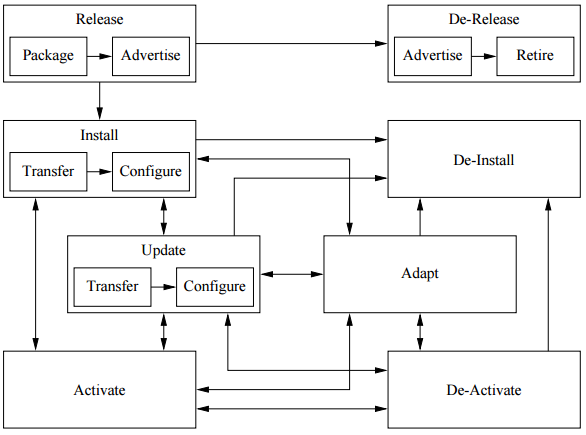
\includegraphics[scale=0.7]{afbeelding/softwareLevenscyclus.png}}
\caption{De levenscyclus van software \citep{carzaniga1998characterization}}
\label{fig:softwareLevenscyclus}
\end{figure}

In theorie zou het deployen van software een eenvoudige klus moeten zijn.
Aangezien software bestaat uit een set van bestanden, zou het deployen van software naar een doelcomputer slechts bestaan uit het kopiëren van de nodige bestanden.
Maar dit is vaak niet het geval.
Volgens \citet{dolstra2006purely} zijn er in de praktijk verschillende oorzaken die aan de basis liggen van een ingewikkeld deployment proces.
Deze oorzaken kunnen in twee grote categorieën ingedeeld worden, namelijk de omgevings- en de onderhoudsproblemen.

\paragraph{Omgevingsproblemen}
In de eerste categorie ligt de nadruk vooral op correctheid.
Voordat de software geïnstalleerd wordt op een doelsysteem, wordt de doelomgeving ondervraagt naar alle eigenschappen: zijn de nodige programma's aanwezig, bestaan alle configuratiebestanden, \ldots .
Als deze eisen niet voldaan zijn, dan zal de software niet werken zoals gewenst.
\citet{dolstra2006purely} haalt enkele concrete voorbeelden aan van omgevingsproblemen:
\begin{itemize}
\item De deployment van software kan een gedistribueerd probleem opleveren.
Software kan afhankelijk zijn van componenten draaiende op externe systemen of van andere processen draaiende op het doelsysteem.  
\item Software is vaak afhankelijk van verschillende andere software componenten. 
Deze afhankelijkheden (dependencies) moeten voor de deployment bepaald worden.
Dit proces is moeilijk en een fout kan pas laat ontdekt worden.
\item De afhankelijkheden moeten compatibel zijn met wat de software verwacht.
Bepaalde versies van een afhankelijkheid zijn compatibel met de software terwijl andere versies dit niet zijn.
Dit komt doordat sommige depencies build-time variaties vertonen.
At build-time worden bepaalde eigenschappen geselecteerd met als gevolg dat de dependency meer of minder functionaliteiten bevat ten opzichte van een vorige build.
\item Sommige software-componenten zijn afhankelijk van specifieke hardware.
Dit kan enkel verholpen worden door op voorhand te controleren welke hardware aanwezig is.
\end{itemize}

Uit deze concrete voorbeelden wordt al snel duidelijk dat er twee problemen zijn: de verschillende eisen van de software moeten geïdentificeerd worden en vervolgens moeten deze eisen voldaan worden in het doelsysteem.

\paragraph{Onderhoudsproblemen}
Naast de verschillende omgevingsproblemen, beschrijft \citet{dolstra2006purely} ook enkele onderhoudsproblemen.
Deze hebben te maken met het feit dat software moet kunnen ``evolueren''.
Om dit te ondersteunen, moeten allerlei actie zoals upgraden en updaten uitgevoerd wordens.
Enkele voorbeelden van zulke acties zijn:
\begin{itemize}
\item Tijdens het verwijderen van software moeten alle componenten verwijderd worden.
Er mogen echter geen componenten verwijderd worden die nog in gebruik zijn door andere software.
\item Ook tijdens het updaten van software moet rekening gehouden worden met andere software.
Het updaten van een component kan voor problemen en failure zorgen in een andere component.
Een DLL-hell wordt best ten alle tijden vermeden.
\item Na het upgraden/updaten van een component, is het soms aangewezen om een rollback uit te voeren.
Zo'n actie kan overwogen worden als na de upgrade belangrijke functionaliteiten van de software niet meer functioneren.
\end{itemize}

\section{Case studies}\label{sec:caseStudies}
Uit de vorige sectie blijkt dat het software deployment proces een uitgebreid en ingewikkeld proces is.
Er moet rekening gehouden worden met verscheidene stappen die elk een eigen doel en functie hebben.
Maar ook met verschillende problemen die kunnen optreden voor, na en tijdens deze stappen.
Door de jaren heen zijn er verschillende technologieën ontwikkeld die het probleem van software deployment aanpakken.
In wat volgt, worden dan ook enkele van deze technologieën besproken en wordt nagegaan op welke manier zij software deployment aanpakken.
Op deze manier wordt een beeld gecreëerd van de mogelijke technologieën die gebruikt kunnen worden om de software van Televic van de producenten naar de gebruikers te krijgen.

%\subsection{Java Beans}
%Enterprise JavaBeans (EJB) zijn een standaard voor het bouwen van server-side componenten.
%De EJB's zijn speciaal ontworpen voor het vereenvoudigen van de deployment.
%\citet{softwareDeployment} beschrijft JavaBeans als eenheden van business logic in een component die uitgevoerd wordt in een container.
%De verschillende containers zorgen voor een abstractie van de hosting omgeving en bieden verscheidene services aan.
%Een JavaBean moet ingepakt worden volgens de specificaties die Sun Microsystems oplegt.
%Met deze standaard is het mogelijk om verschillende management en deployment tools te schrijven die de EJB's kunnen beïnvloeden.
%Enterprise JavaBeans worden ingepakt in de standaard Java JAR file, samen met een XML deployement descriptor.
%De descriptor beschrijft de verschillende eigenschappen van de bijhorende EJB.
%
%De Enterprise JavaBeans zijn volgens \citet{softwareDeployment} fijnkorrelige en taalafhankelijke oplossing voor het deployment probleem.
%Door het isoleren van de Beans door middel van een gestandaardiseerde container interface zullen Enterprise JavaBeans zo een oplossing vinden voor het deployment probleem.
%Hierdoor moeten de EJB's zodanig ontworpen worden dat ze voldoen aan de eisen van de interface.
%Enterprise JavaBeans hebben geen idee van het op afstand installeren van componenten.
%Een groot probleem bij EJB's is dat referenties naar afhankelijke beans gebeurd via niet unieke namen.
%Twee verschillende beans met eenzelfde naam moeten hierdoor manueel herladen worden zodanig dat de bindings up-to-date zijn \citep{rutherford2002reconfiguration}.
\subsection{Electric cloud}
%%% TODO
%http://electric-cloud.com/wp-content/uploads/Ovum-Decision-Matrix-Selecting-DevOps-Release-Management-Solution-2016-2017-print.pdf
%https://www.gartner.com/doc/reprints?id=1-3DSWYP2&ct=160801&st=sb
Electric cloud is een bedrijf opgericht in 2002 met een focus op application release automation (ARA).
Hun product, ElectricFlow, is ontworpen om gebruikers in staat te stellen om het beschikbaar stellen, het bouwen en het verspreiden van mutlitiered applicaties te vereenvoudigen.
Dit allemaal aan de hand van de model-driven architectuur \citep{gartner}.
\citet{electricflow} beschrijft ElectricFlow als een enterprise-grade DevOps Release Automation platform.
Met behulp van de model-driven aanpak is het mogelijk voor gebruikers om meerde pipelines en releases over verschillende infrastructuren te coördineren op een eenvoudige manier.

De kern van ElectricFlow bestaat uit een web-based systeem dat gebruikt wordt voor de automatie en het onderhouden van het bouw-, test-, deployment en releaseproces.
Het automatieplatform bestaat uit een drie-lagen architectuur, een web interface en mogelijkheden om build en release analyses uit te voeren.
De drie-lagen architectuur van ElectricFlow bestaat uit:
\begin{itemize}
\item \textbf{ElectricFlow Server}: een server die instaat voor het managen van resources, commando's en het generen van rapporten.
\item \textbf{Databank}: een databank die instaat voor het opslaan van commando's, meta-data en logfiles.
\item \textbf{Agents}: verschillende agenten die instaan voor het uitvoeren van commando's, het monitoren van statussen en het verzamelen van resultaten.
\end{itemize}
Figuur~\vref{fig:electricflowArchitecture} geeft een architecturaal overzicht weer van ElectricFlow.
In de figuur zijn de verschillende lagen zichtbaar samen verschillende andere tools die vervat zitten in het automatisatie platform \citep{electricflow}.

\begin{figure}[!ht]
\centering
\makebox[0pt]{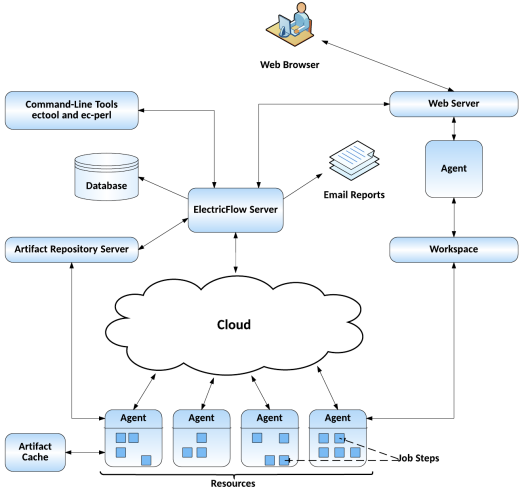
\includegraphics[scale=0.9]{afbeelding/electricflowArchitecture.png}}
\caption{ElectricFlow Architectuur \citep{electricflow}}
\label{fig:electricflowArchitecture}
\end{figure}

Om ElectricFlow te gebruiken voor bouw en test automatie, is het nodig om de volgende objecten te creëren, te configureren en bij te houden.
\begin{itemize}
\item \textbf{Project}: een project in ElectricFlow dient als container waarin procedures, stappen, workflows, \ldots zitten.
Op deze manier is het mogelijk om een scheiding te creëren tussen projecten die bijvoorbeeld een ander doel hebben.
\item \textbf{Resource}: een resource wordt gedefinieerd als een agent machine waar stappen in uitgevoerd kunnen worden.
\item \textbf{Procedures}: procedure en stappen worden gebruikt om taken in ElectricFlow te definiëren.
Een procedure bestaat uit één of meerdere stappen waarbij in ieder stap een commando of script wordt uitgevoerd.
\item \textbf{Workflow}: een workflow stelt de gebruiker in staat om build-test-deploy levenscycli te definiëren.
Zo wordt het managen van verschillende procedures en stappen in een project eenvoudiger.
\end{itemize}

Met ElectricFlow is het mogelijk om verscheiden applicaties op een autonome wijze te verschepen naar de gebruikers.
Hierbij kan door middel van een procedure een gepersonaliseerde afhandeling plaatsvinden.
Door gebruik te maken van de verscheidene projecten is het mogelijk om de release van verschillende applicaties op een geordende manier aan te pakken. 
Verder wordt niks vermeld over hoe omgegaan wordt met installaties en updates die slecht zijn afgelopen.

\subsection{Redhat package manager}
In Linux wordt de Redhat package manager (RPM) het vaakst gebruikt voor de deployment van software.
Met hulp van de RPM is het mogelijk om enkele operaties uit te voeren zoals onder andere installatie, updaten, \ldots .
De operaties worden ondersteund door een databank die alle informatie en details van de geïnstalleerde pakketten bevat.
Een RPM pakket bestaat uit executables gecombineerd met configuratie bestanden en documentatie.
Doordat een pakket executables bevat, zal een pakket gekoppeld zijn aan het besturingssysteem van de host \citep{bailey1997maximum}.
Naast de RPM files bevat een pakket verschillende scripts geschreven in de standaard Unix scripting taal.
De verscheidene scripts zijn ingedeeld in sets horende bij een specifieke taak.
Bij een error moet een roll back uitgevoerd worden.
Dit is de taak van de script schrijver \citep{softwareDeployment}.

De Redhat Package Manager is een grofkorrelige, taal onafhankelijke maar besturingssysteem afhankelijke oplossing.
Het grootste probleem van RPM schuilt in de afhankelijkheden tussen de pakketten.
Niet alle afhankelijkheden zijn explicite gemodelleerd en de afhankelijkheden die wel gemodelleerd zijn, zijn gevormd met de nadruk op de inhoud en niet op de pakketten zelf \citep{softwareDeployment}.  

\subsection{ATLAS}\label{sec:ATLAS}
ATLAS is één van de vier grote experimenten bij de Large Hadron Collider (LHC) in CERN (de Europese organisatie voor nucleair onderzoek).
Het is een algemeen deeltjesfysica experiment onderhouden door een internationale samenwerking met als doel het exploiteren van de mogelijkheden van de Large Hadron Collider.
Fysici testen de voorspellingen van het Standaard Model \cite{standardModel} wat kan leiden tot grote ontdekkingen zoals het Higgs  boson \cite{atlas}.

Om in de ATLAS samenwerking om te gaan met de grote hoeveelheid bronnen, is er een volledig automatisch installatie systeem ontworpen voor het LCG/EGEE project, LHC Computing Grid/Enabling Grids for E-sciencE \citep{bird2005lhc}. 
\citet{salvo2008atlas} beschrijft de architectuur van het ontworpen systeem.
Het ontwerp van het installatie systeem werd gebaseerd op het Light Job Submission Framework for installation, ook wel LJSFi.

\begin{figure}[!ht]
\centering
\makebox[0pt]{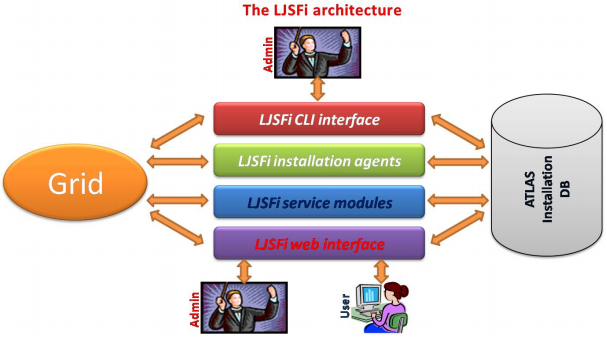
\includegraphics[scale=0.7]{afbeelding/ljsfiArchitectuur.png}}
\caption{LJSFi Architectuur \citep{salvo2008atlas}}
\label{fig:ljsfiArchi}
\end{figure}

De architectuur van het framework is zichtbaar in Figuur~\ref{fig:ljsfiArchi}.
Het framework vormt een dunne laag over de middleware van Grid.
De kern van het systeem bestaat uit de installatie database en de command line interface (CLI).
De laatste zorgt voor de interacties met de Grid middleware.
Met hulp van de installatie database kan de CLI verschillende taken en job informatie opslaan.
Aan de hand van deze informatie kunnen installaties uitgevoerd worden.
De installatie databank staat in contact met alle componenten van het framework.
Zo kan de status van verscheidene acties en configuraties van verschillende taken opgeslagen worden.

Naast deze twee grote componenten bevat LJSFi service modules en extensies waarmee installatie aanvragen afgehandeld worden.
Het systeem bevat drie verschillende componenten die horen bij de LJSFi service modules:
\begin{itemize}
\item \textbf{RAI module} De Request An Installation module dient als web interface voor het ontvangen van user-driven installatie aanvragen.
\item \textbf{AIR module} De Automatic Installation Requester schiet in actie als de software release aangeduid staan als productie of veroudert en als de release aangeduid staat met de parameter auto-installatie.
De module zal respectievelijk de software installeren of verwijderen op alle sites waar de software tag nog niet aanwezig is.
Door de AIR module periodiek te gebruiken, zullen de nodige aanvragen snel afgehandeld worden.
\item \textbf{InAgent module} Met de InAgent module wordt het mogelijk om volledig geautomatiseerde installatieprocessen te voorzien.
Iedere 10 minuten wordt de Installation database gelezen en via de CLI interface worden de nodige installatieprocessen opgestart.
Elk installatieproces wordt bijgestaan door een installation agent.
De agent zal instaan voor het updaten van de Installatie database met real-time informatie die zichtbaar is online.
\end{itemize}

Naast de verscheidene automatische services biedt LJSFi enkele gebruiker services aan.
Een gebruiker kan zich subscriben voor bepaalde acties op een doel systeem.
Als deze actie wordt uitgevoerd dan krijgt de gebruiker een mail.
Hiernaast kan een gebruiker een software release vastpinnen zodat deze niet verwijderd kan worden door het systeem.

Het installatieproces wordt uitgevoerd in drie verschillende stappen.
In een eerste stap wordt een site check uitgevoerd door een pilot job naar de site te sturen.
Als de check succesvol uitgevoerd wordt, kan het installatieproces beginnen.
De acties tijdens het installatieproces worden uitgevoerd door softwaremanagement scripts.
Op het einde van het proces, haalt het systeem de job output en exit code op.
De laatste wordt opgeslagen in de Installation database.

\citet{Obreshkov2008244} bespreekt hoe het ATLAS project te werk gaat bij het inpakken van alle nodige software.
Het ATLAS project gebruikt CMT \citep{cmt} als configuratie manager.
Met behulp van een configuratie bestand weten verscheidene tools hoe ze een pakket moeten afhandelen.
\citet{packAtlas} spreekt ook over CMT als informatiebron voor het ophalen van meta-data.
Aan de hand van deze data kan een Pacman pakket geproduceerd worden.
Met behulp van een ``Pacman file'' is geweten hoe de ingepakte software behandelt moet worden.

De LJSFi architectuur is een architectuur die om kan gaan met een grote hoeveelheid pakketten.
Door gebruik te maken van de modules is het mogelijk om de verschillende pakketten te installeren en te verwijderen op een grote schaal zonder dat menselijke interactie nodig is.
Hierbij zorgt CMT voor de nodige meta-data waardoor installatietools niet afhankelijk zijn van de mens.
Een nadeel aan deze architectuur is dat het gebruik van Grid nodig is om de LJSFi architectuur in te bouwen.
Verder wordt in de lectuur niet ingegaan op welke wijze er wordt omgegaan met een fout tijdens het installatieproces of het verwijderproces.
Het enige dat hierover vermeld wordt is dat de exit code van de job wordt opgeslagen in de databank.

\subsection{ORYA}\label{sec:ORYA}
\citet{lestideau2003providing} legt uit hoe ORYA (Open enviRonment to deploY Applications) verschillende deployment functionaliteiten aanbiedt aan gedistribueerde, autonome entiteiten zoals workstations en servers.
Aan de hand van een deployment PSEE \citep{belkhatir2007adele} wordt het mogelijk om het installatieproces te automatiseren.

In het ontwerp van ORYA worden er drie verschillende entiteiten besproken die nodig zijn om het automatische installatieproces mogelijk te maken.
\begin{itemize}
\item \textbf{Applicatie Server} De applicatie server bevat de informatie nodig voor de installatie.
Hieronder bevindt zich onder andere een pakket met de nodige resources en een manifest waarin de afhankelijkheden, beperkingen en kenmerken staan.
\item \textbf{Target} De target is het doel waarop de deployment uitgevoerd wordt.
Iedere target wordt beschreven door de verschillende applicaties die al aanwezig zijn en de fysische beschrijving.
\item \textbf{Deployment Server} De deployment server vormt de kern van de deployment omgeving en staat in voor het uitvoeren van de deployments. 
De deployment server zoekt de nodige pakketten, voert een transfer van de pakketten uit en installeert de applicatie.
Op het einde moet de deployment server garanderen dat vorige programma's correct blijven functioneren.
\end{itemize}

\citet{lestideau2003providing} beschrijft verder de verschillende modellen die gehanteerd worden om een succesvolle deployment uit te voeren.
In Figuur~\vref{fig:deploymentModel} is het deployment proces model terug te vinden.
Een deployment proces zal bestaan uit verschillende basis activiteiten en deployment processen.
Iedere activiteit wordt uitgevoerd door een agent.

\begin{figure}[!ht]
\centering
\makebox[0pt]{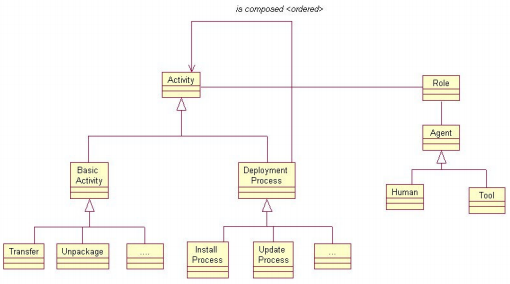
\includegraphics[scale=1]{afbeelding/deploymentModelORYA.png}}
\caption{Deployment proces model \citep{lestideau2003providing}}
\label{fig:deploymentModel}
\end{figure}

Een toegepast voorbeeld van een deployment aan de hand van dit model is terug te vinden in Figuur~\vref{fig:deploymentVoorbeeld}.
Een basis activiteit wordt voorgesteld aan de hand van een grijze rechthoek en een deployment proces aan de hand van een witte rechthoek.
In het voorbeeld zijn dus vier deployment processen aanwezig en 3 basis activiteiten.

\begin{figure}[!ht]
\centering
\makebox[0pt]{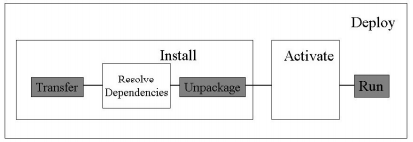
\includegraphics[scale=0.7]{afbeelding/deploymentVoorbeeld.png}}
\caption{Voorbeeld van een deployment \citep{lestideau2003providing}}
\label{fig:deploymentVoorbeeld}
\end{figure}

Aan de hand van deze structuur wordt het mogelijk om het volledige deployment proces voor te stellen.

%\subsection{Unix}
%\citet{dolstra2006purely} bespreekt Nix deployment systeem omgaan met het deployment probleem.
%Nix houdt verschillende componenten bij in de component store waarbij iedere component een set van bestanden is.
%De componenten worden van elkaar gescheiden door een unieke naam.
%Dit wordt bekomen door een cryptografische hash op te nemen in de naam.
%Unix biedt geen software deployment aan.
%Het biedt verscheidene mechanismen aan waarmee verschillende deployment beleid beschikbaar worden.
%Met de volgende deployment models is het mogelijk om in Unix de Unix expressies (de bouwstenen van de Unix componenten) te verspreiden:
%\begin{itemize}
%\item \textbf{Handmatige download} Een gebruiker kan zelf pakketten downloaden in de vorm van tar archieven, deze zelf uitpakken en vervolgens installeren.
%Deze strategie is arbeidsintensief en maakt het moeilijk om alles up-to-date te houden. 
%\item \textbf{Updaten aan de hand van een versie management systeem} Een andere strategie is het gebruik van een versie management systeem.
%Hiermee is het up-to-date houden van de pakketten zeer eenvoudig.
%\item \textbf{Kanalen} Een verdere uitbreiding zijn de kanalen.
%Een kanaal is een URL naar een tar archief die de nodige Unix expressies bevat.
%Met deze strategie is het even eenvoudig om pakketten te installeren en up-to-date te houden.
%\item \textbf{One-click installatie} Als er enkel één pakket geïnstalleerd moet worden, dan is de one-click installatie de eenvoudigste optie.
%Via de website van de verdeler kan een link gebruikt worden om het nodige pakket te installeren.
%\end{itemize}

\subsection{Ansible}
Als laatste case studie wordt Ansible besproken.
Ansible is een open source IT configuratie management, deployment en organisatie tool.
De architectuur van Ansible bestaat uit een agentless push model.
Dit wil zeggen dat er geen additionele software nodig is op de client toestellen.
Dit wordt behaald door gebruik te maken van de remote manegement frameworks aanwezig op de toestellen, SSH voor Linux en Unix en WinRM voor Windows.
Door geen agents te gebruiken, zal Ansible geen resources gebruiken zolang de Ansible het systeem niet aan het gebruiken is \citep{ansible}.

\citep{ansible} beschrijft verder dat Ansible gebruik maakt van \emph{Playbooks} voor de organisatie van de IT omgevingen.
Playbooks zijn YAML\footnote{Een human-readable data serialisatie taal (Een superset van JSON)} definities van taken die beschrijven hoe een taak moet geautomatiseerd worden.
Een Playbook bestaat uit een aantal ``plays'' die uitgevoerd kunnen worden op een set van hosts, ook wel een ``inventory'' genoemd.
Iedere play bestaat uit een set van taken die op een subset van de inventory uitgevoerd kan worden.
Een task zelf voert een Ansible module uit\footnote{Een klein stuk code met een specifieke taak}.

Hiernaast is het mogelijk om de mogelijkheden van Ansible uit te breiden.
Modules kunnen zelf geschreven worden in eender welke taal met als enige beperking dat een JSON bestand als input moet gegeven worden en dat een JSON bestand gegenereerd moet worden.
De inventory van een Playbook kan dynamisch ontdekt worden at runtime.

In tegenstelling tot ATLAS en Electric Cloud bevat Ansible geen agenten die gebruikt worden om het deployment proces in goede banen te leiden.
Het is wel mogelijk om het proces te beïnvloeden door gebruik te maken van de Playbooks.
Door gebruik te maken van modules is het in Ansible mogelijk om de functionaliteiten uit te breiden.
Wederom is het niet duidelijk wat er gebeurt mochten er fouten optreden tijdens het installatieproces of updateproces.

\section{Recovery na fouten}\label{sec:rollback}
Tijdens de bespreking van het probleem in Sectie~\vref{sec:probleem} werd al aangehaald dat een soort van rampenplan voorzien moet worden.
Zowel omgevingsproblemen als onderhoudsproblemen (zie Sectie~\vref{sec:softwareLevenscyclus}) kunnen tijdens één van de toestanden in de deployment levenscyclus optreden.
Voor Televic is het niet wenselijk dat een probleem tijdens één van deze toestanden ervoor zorgt dat hun software niet meer correct functioneert aangezien dit kan leiden tot het stilleggen van de productie.
Daarom wordt in de volgende secties verschillende mechanismen besproken waarmee de verscheidene problemen aangepakt kunnen worden.
In wat volgt, wordt vooral rekening gehouden met mechanismen die gebruikt kunnen worden als het probleem zich al voor heeft gedaan.
Deze strategieën zullen typisch proberen terug te keren naar een vorige correct werkende toestand van de software.
De actie waarbij wordt teruggekeerd naar een vorige toestand wordt ook wel rollback genoemd.

\subsection{Rollback strategieën}
\citet{srinivasan2004flashback} spreekt over drie manieren waarop rollback strategieën geïmplementeerd worden in hedendaagse systemen.
Checkpointing, main-memory transactions en software rejuvination zijn strategieën die vaak gebruikt zijn.

\paragraph{Checkpointing}
Checkpointing is een eenvoudige recovery strategie.
De toestand van een programma wordt periodiek opgeslagen in een bestand op een extern opslagmedium.
Deze kan, na het falen van het programma, gebruikt worden om te herstellen van fouten \citep{plank1994libckpt}.
Bij een checkpointing systeem wordt de volledige toestand van het programma opgeslagen.
Dit zorgt voor een verhoogde overhead waardoor het niet mogelijk is om frequent een checkpoint uit te voeren \citep{srinivasan2004flashback}.

Door gebruik te maken van incrementele checkpoints is het evenwel mogelijk om dit probleem aan te pakken.
Enkel de veranderingen van de laatste checkpoint worden opgeslagen in een nieuwe checkpoint.
Het deel dat niet is aangepast, kan hersteld worden aan de hand van de vorige checkpoint.
Dankzij deze strategie is het mogelijk om de hoeveelheid data die moet worden opgeslagen te verkleinen.
Hierdoor zullen wel verschillende recovery bestanden nodig zijn.
Het is aangewezen om op regelmatige tijdstippen de verschillende recovery bestanden samen te voegen tot één bestand \citep{plank1994libckpt, elnozahy2002survey}.

\paragraph{Main-memory transactions}
Een andere rollback strategie zijn de main-memory transactions.
Systemen die deze transacties ondersteunen bezitten vaak de mogelijkheid om terug te keren naar een vorig executie punt.
Om deze strategie te kunnen implementeren, moeten applicaties gebruik maken van het transactieprogrammeermodel, waardoor de keuzevrijheden van de programmeur beperkt worden \citep{srinivasan2004flashback}.

\paragraph{Software rejuvenation}
\citet{huang1995software} definieert software rejuvination als volgt:
\begin{displayquote}
``Software rejuvenation is the concept of gracefully terminating an application and immediately restarting it at a clean internal state.''
\end{displayquote}
Tijdens het langdurig uitvoeren van een programma treedt \emph{process aging} op.
Door geheugenlekken, niet vrijgegeven bestandlocks, data corruptie, \ldots zal de performantie van het uitvoerende programma aangetast worden waardoor het programma uiteindelijk faalt.
Door het heropstarten van de applicatie worden eventuele fouten uit het systeem gehaald en wordt de software verjongd.
De meeste studies over software rejuvenation focussen vooral op het herstarten van de volledige applicatie en werken dus niet op een fijnkorrelige schaal \citep{srinivasan2004flashback}.

\subsection{Virtualisatie}\label{sec:virtualisatie}
Door middel van virtualisatie wordt de complexiteit die ontstaat door de interactie tussen het programma, de installatieomgeving en de uitvoeringsbeperkingen gelimiteerd.
Door het creëren van een perfecte omgeving komen deze problemen niet voor.
Er zijn verschillende voordelen gekoppeld aan het gebruiken van een virtuele machine (VM).
Bijvoorbeeld, besturingssystemen op verschillende hardware platformen eisen verschillende drivers en deze drivers hebben misschien afhankelijkheden op een bepaalde firmware en BIOS.
Een guest OS draaiende op een virtuele machine heeft deze eisen niet \citep{shumate2004implications}.

\begin{figure}[!ht]
\centering
\makebox[0pt]{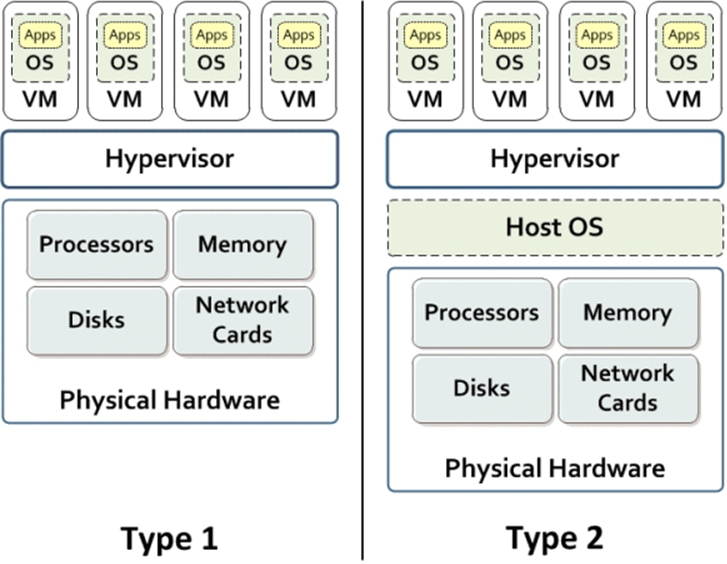
\includegraphics[scale=0.4]{afbeelding/hypervisors.png}}
\caption{Typer 1 hypervisor in vergelijking met een type 2 hypervisor \citep{hypervisors}}
\label{fig:hypervisors}
\end{figure}

Met virtualisatie is het mogelijk om van één computer meerder computers te maken.
Dit kan bereikt worden door gebruik te maken van een speciaal programma (een hypervisor).
Volgens \citet{fenn2008evaluation} bestaan er twee types hypervisors:
\begin{itemize}
\item \textbf{Type 1} hypervisors zorgen voor een directe interface naar de host hardware.
Er is typisch één virtuele machine met speciale privileges die de andere virtuele machines onderhoudt.
\item \textbf{Type 2} hypervisors draaien als een normaal programma in het host besturingssysteem.
Iedere virtuele machine draait dan als proces in het host besturingssysteem.
\end{itemize}
Deze twee types zijn zichtbaar in Figuur~\vref{fig:hypervisors}.

Een virtuele machine bevat een volledig besturingssysteem.
Een gevolg hiervan is dat het uitvoeren van handelingen (zoals opstarten, afsluiten, kopiëren, \ldots) lang duren.
Hiernaast moet tijdens het instellen van een virtuele machine een volledig besturingssysteem geïnstalleerd worden.
De tijd die nodig is om een VM in te stellen neemt hierdoor drastisch toe.
Aangezien een virtuele machine een volledig besturingssysteem omvat, heeft deze ook de resources nodig om correct te kunnen functioneren.
Om verschillende virtuele machines naast elkaar te kunnen laten draaien, moet de host voldoende RAM, CPU en harde schijf ruimte hebben.
Door gebruik te maken van een virtuele machine wordt een veilige omgeving gecreëerd maar dit neemt kostbare tijd en resources in beslag.

\begin{figure}[!ht]
\centering
\makebox[0pt]{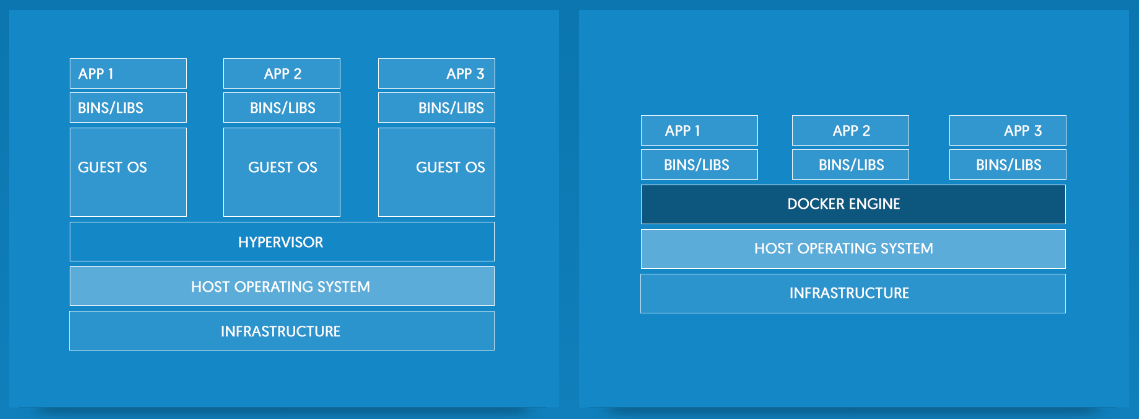
\includegraphics[scale=0.5]{afbeelding/dockerVsVM.png}}
\caption{Architectuur van Virtuele Machine ten opzichte van Docker \citep{dockerMain}}
\label{fig:VMvsDocker}
\end{figure}

\subsection{Docker}\label{sec:docker}
Virtualisatie is niet de enige techniek die gebruikt kan worden om rollbacks te vermijden.
Docker containers is een technologie waarmee een stuk software wordt ingepakt in een volledig filesysteem dat alle benodigdheden bevat om correct te functioneren.
Hierdoor zal de software overal op eenzelfde manier draaien, ongeacht de omgeving \citep{dockerMain}.
Docker containers zijn niet hetzelfde als virtuele machines.
In de vergelijking \citep{dockerEbook} worden virtuele machines voorgesteld als huizen terwijl Docker containers worden voorgesteld als appartementen.

De huizen staan volledig op zichzelf en bieden bescherming tegen ongewenste gasten.
Ze hebben een eigen infrastructuur met hun eigen water, verwarming, \ldots .
Hiernaast zal ieder huis op zijn minste een badkamer, living, slaapkamer en keuken hebben.
Het vinden van een klein huis is een ganse klus en vaak zal een huis meer bevatten dan nodig is want dat komt door de manier waarop huizen gebouwd worden.

Appartementen bieden ook bescherming tegen ongewenste gasten, maar zij zijn gebouwd rond een gemeenschappelijke infrastructuur.
Het appartementsgebouw biedt gemeenschappelijk water, verwarming, \ldots  aan, aan elk appartement.
Elk appartement verschilt ook nog van grootte.
Er bestaan kleine appartementen maar ook grote met meerder slaapkamers.
Men huurt enkel hetgeen dat nodig is.

In Figuur~\vref{fig:VMvsDocker} zijn de architecturen van virtuele machines en Docker terug te vinden.
Het verschil tussen beiden wordt al snel duidelijk.
Een virtuele machine zal typisch de applicatie, de nodige binaries en bibliotheken en een volledig besturingssysteem bevatten.
Een container bevat de applicatie en de verschillende dependencies maar de kernel wordt gedeeld met alle andere containers en gedragen zich als een geïsoleerd proces in de user space van het host besturingssysteem.

\citet{chamberlain2014using} bespreekt kort hoe Docker werkt.
Docker is een platform dat gebruik maakt van de Linux Containers (LXC de user-space control package voor Linux Containers) om software te encapsuleren.
LXC is een virtualisatie techniek waarmee virtuele omgevingen in Linux opgebouwd kunnen worden.
De containers zullen processen van elkaar sandboxen zodanig dat een proces een ander niet kan beïnvloeden \citep{merkel2014docker}.
Docker zal de LXC software uitbreiden waardoor deployment, distributie en versioning mogelijk wordt.
Naast LXC gebruikt Docker AuFS (Advanced Multi-Layered Unification Filesystem) als het filesysteem voor de containers.
Doordat het filesysteem gelaagd is, is het mogelijk om verschillende filesystemen over elkaar te leggen.

\citet{merkel2014docker} vergelijkt de twee virtualisatie technieken en bespreekt de verschillende tussen de twee.
Bij virtuele machines moet voor iedere virtuele machine een besturingssysteem geïnstalleerd worden.
Al deze besturingssystemen verbruiken RAM, CPU en bandbreedte.
Containers zullen piggybacken op het bestaande host besturingssysteem.
Hierdoor zal het resource gebruik efficiënter zijn.
Een container is goedkoop waardoor het creëren en verwijderen van containers een snelle operatie.
Dit komt omdat er enkel een proces moet afgesloten worden in tegenstelling tot het afsluiten van een volledig besturingssysteem.
Een voordeel van de VMs ten opzichte van Docker is hun maturiteit.
VMs bestaan langer en hebben zichzelf kunnen bewijzen in verschillende situaties.

\section{Deployment strategieën}\label{sec:deployment}
%%% TODO herschrijven
Voordat software bij een gebruiker geïnstalleerd of geüpdatet kan worden, moet de software eerst bij de gebruiker geraken.
Er kan op twee manieren naar dit proces gekeken worden:
\begin{itemize}
\item Wat wordt er precies verzonden naar de gebruiker?
\item Wie krijgt de software als eerste?
\end{itemize}
In de volgende secties worden deze twee verschillende focussen verder besproken.

\subsection{Data focus}
\citet{deploymentMethods} haalt drie methodes aan om software te deployen:
\begin{itemize}
\item disk image-based deployment
\item behavior-based deployment
\item package-based deployments
\end{itemize}
Bij disk image-based deployment worden de software en het besturingssysteem op eenzelfde moment naar de target node verzonden.
Er zullen verschillende image-servers aanwezig zijn die elk een service aanbieden.
Zo zal de image-server van software A een andere image-server zijn dan de image-server die software B gebruikt.
Het voordeel van deze strategie is dat, zolang de hardware en software vereisten voldaan zijn, de deployment bestaat uit een simpele read-write operatie.
Maar, zoals \citet{deploymentMethods} al aangeeft, is deze methode niet flexibel.
Enkel software die op voorhand werd geconfigureerd op de image-server kan worden gedeployed.
Gebruikers met speciale noden kunnen moeilijk worden geholpen.
Voor Televic is flexibiliteit een hoofddoelstelling.
Iedere node bevat verschillende hardware en is verschillend geconfigureerd.
Een disk image-based deployment zal hierdoor niet gebruikt kunnen worden.
Het basisidee achter behavior-based deployment is het opnemen van de schijfoperaties tijdens het deployen.
Als geweten is welke bestanden aangepast, gecreëerd zijn, ... dan kan het proces nagebootst worden op andere nodes \citep{deploymentMethods}.
Zo een proces nabootsen is moeilijk.
Kerneloperaties moeten getraceerd worden.
Deze methode biedt een verhoogde flexibiliteit aan ten opzichte van de disk image-based deployment maar dit is nog niet voldoende om deployments uit te voeren die uniek zijn per node.
De laatste techniek die \citet{deploymentMethods} aan haalt is package-based deployment.
Met behulp van een batch file, waarin alle nodige commando's aanwezig zijn, kan een installatie pakket gedeployed worden naar een target node.
Door het gebruik van een batch file wordt de flexibiliteit van de deployment verhoogd.

\subsection{User focus}
De geproduceerde software moet bij verschillende gebruikers terecht komen.
Een eenvoudige oplossing zou zijn dat slechts één gebruiker per keer geholpen wordt en dat iedere gebruiker zijn beurt afwacht.
Zo'n oplossing is misschien doenbaar mochten slechts een handvol gebruikers de applicatie nodig hebben maar dit is vaak niet het geval.
\citet{patterson2008data} haalt verschillende argumenten aan voor het distribueren van deze service en haalt enkele punten aan (betrouwbaarheid, bandbreedte en lage wachttijden) waar rekening mee moet gehouden worden alvorens een ontwerpbeslissing genomen wordt.
Zoals \citet{patterson2008data} aanhaalt, is het belangrijk dat alle gebruikers ten alle tijden de service kunnen gebruiken.
Hiernaast moet er rekening gehouden worden met de deployment strategie.
\citet{munch2012software} spreekt over verschillende strategieën om software uit te brengen:
\begin{itemize}
\item \emph{Big-bang}: iedere gebruiker van de applicatie zal op eenzelfde moment overschakelen van de oude naar de nieuwe software. 
Hierdoor wordt vermeden dat verschillende afdelingen met een andere versie van de software werken. 
Een nadeel is dat voldoende support aanwezig moet zijn om mogelijke problemen op te lossen.
\item \emph{Gefaseerd}: de nieuwe software zal bij een gefaseerde deployment enkel toegepast worden in specifiek geselecteerde projecten.
Als deze strategie voor een verlengde periode wordt toegepast, zullen verschillende versies van de software continu aanwezig zijn onder de gebruikers.
\end{itemize}
Aan beide strategieën zijn zowel voor- en nadelen gekoppeld.
Zo zal de big-bang strategie niet voordelig zijn om uit te voeren als de gebruikers verspreid zitten over de wereld.
Door het tijdsverschil zal de deployment bij sommige gebruikers plaatsvinden tijdens de werkuren en bij anderen midden in de nacht.
Het voordeel van de big-bang strategie is dat alle doelsystemen op een korte periode omgeschakeld worden naar de nieuwe versie van de applicatie. 
Het gebruik van de gefaseerde strategie kan het probleem met de tijdszones omzeilen maar deze strategie is ook niet ideaal aangezien het omschakelen van de software naar de nieuwe versie lang kan duren.
Een hybride oplossing is hier dus aangewezen.

\section{Architecturen}
Tot op heden werd vooral gekeken naar mogelijke technologieën en tools die gebruikt kunnen worden voor het verspreiden van software.
In de komende secties worden enkele architecturen aangehaald die ook een oplossing bieden voor het verspreiden van software.
Met een architectuur is het mogelijk om zelf verscheidene ontwerp- en implementatiebeslissingen te nemen.
Zo ligt de programmeertaal niet vast en kan een taal gekozen worden die besturingssysteem onafhankelijk is.
In de volgende secties wordt vooral gekeken of de architecturen een schaalbare oplossing bieden voor het deployment proces.

\subsection{Drie lagen architectuur}
Volgens \citet{micro} is het mogelijk om een applicatie in te delen in drie logische groepen of ook wel lagen.
Het gebruik van een laag stelt de ontwerper in staat om verscheidene taken van elkaar te onderscheiden waardoor het eenvoudiger is om een laag te ontwerpen die herbruikbaar is.
Figuur~\vref{fig:threeLayer} toont welke drie basis lagen gebruikt worden om de architectuur op te bouwen.
Hierbij wordt de presentatie laag gebruikt om alle functionaliteiten die instaan voor het onderhouden van de gebruikersinteracties met het systeem te groeperen.
De bussiness laag encapsuleert alle relevante bussiness logica die de kern van het systeem bevat.
De laatste laag, de data laag, voorziet toegang tot verschillende databronnen binnen in het netwerk maar ook daarbuiten.
 
\begin{figure}[!ht]
\centering
\makebox[0pt]{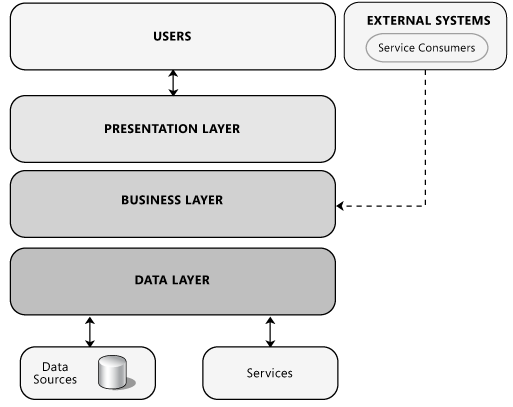
\includegraphics[scale=0.7]{afbeelding/threeLayer.png}}
\caption{Drie lagen architectuur \citep{micro}}
\label{fig:threeLayer}
\end{figure}

Het gebruik van deze architectuur gaat gepaard met enkele voordelen.
Zo zorgt het gebruik van lagen ervoor dat het aanpassen van één laag amper of geen invloed heeft op de andere lagen.
Verder zorgt het opdelen van de applicatie en database functionaliteiten ervoor dat beter load balancing kan worden toegepast.
In de verschillende lagen is het mogelijk om voldoende veiligheidsmaatregelen toe te passen zonder de gebruikers te hinderen.
Figuur~\vref{fig:threeLayerExample} geeft weer op welke wijze de architectuur gebruikt kan worden om een applicatie hosten.

\begin{figure}[!ht]
\centering
\makebox[0pt]{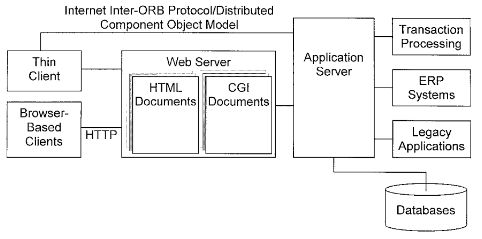
\includegraphics[scale=1]{afbeelding/threeLayerExample.png}}
\caption{Voorbeeld van een drie lagen architectuur \citep{hanson2000client}}
\label{fig:threeLayerExample}
\end{figure}

Het verspreiden van software kan met deze architectuur op een eenvoudige manier gerealiseerd worden.
Clients kunnen verbinding maken met een web server.
Vanuit een browser is het vervolgens mogelijk om verschillende software componenten te combineren tot één geheel die naar de gebruiker verscheept wordt voor installatie.
De web server zorgt voor de nodige flexibiliteit waarbij het voor een gebruiker mogelijk is om vanuit een browser de te installeren software zelf te selecteren.
De software kan bij de gebruiker geraken maar de architectuur biedt geen mogelijkheden aan die toestaan om de software te installeren.
Hiervoor is echter ondersteuning nodig die niet is opgenomen in de architectuur.
Hiernaast laat de architectuur ook een groeiend aantal gebruikers toe.
Iedere laag kan redundant gemaakt worden waarbij meerdere server van eenzelfde laag parallel naast elkaar kunnen draaien.
De drie lagen architectuur voorziet voldoende flexibiliteit en schaalbaarheid maar logica voor het opvangen van fouten tijdens het installatieproces en updateproces is niet aanwezig.

\subsection{Software dock architectuur}\label{sec:softwareDock}
\citet{hall1999cooperative} bespreekt een interessante architectuur die gebruikt kan worden voor het verspreiden van software.
Het Software Dock research project creëerde een raamwerk om de samenwerking tussen software producenten en gebruikers te verbeteren.
In Figuur~\vref{fig:softwareDock} wordt de ontworpen architectuur voorgesteld.
Er worden twee verschillende componenten gedefinieerd waarmee de producenten en gebruikers voorgesteld worden.
In de architectuur worden de verschillende producenten voorgesteld aan de hand van een release dock en worden de gebruikers voorgesteld als een field dock.
Aan deze docks worden verschillende agenten gekoppeld.
Elke agent hoort typisch bij één stap uit de software levenscyclus die besproken werd in Sectie~\ref{sec:softwareLevenscyclus}.
Naast de verschillende docks wordt ook een wide-area eventsysteem gedefinieerd.
Met dit systeem wordt de communicatie tussen de docks aangeboden.
\citet{hall1997architecture} bespreekt in detail hoe de Software Dock architectuur gebruikt kan worden voor het verspreiden van software.

\begin{figure}[!ht]
\centering
\makebox[0pt]{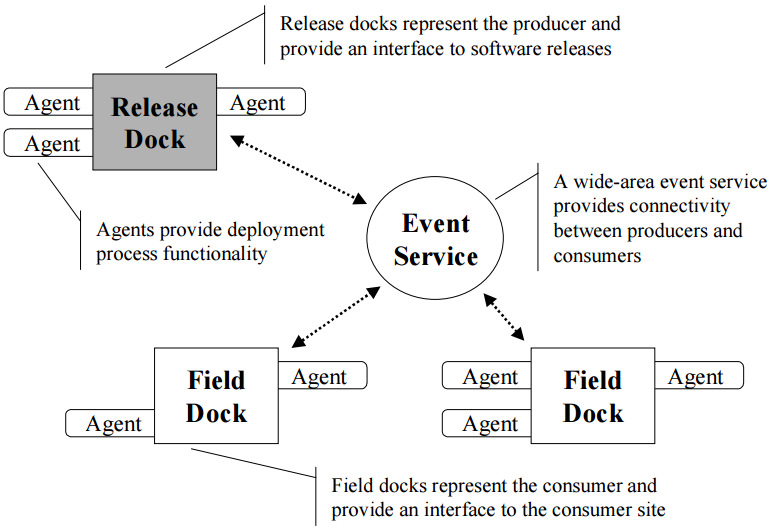
\includegraphics[scale=0.5]{afbeelding/softwareDockArchitectuur.png}}
\caption{Software Dock Architectuur \citep{hall1999cooperative}}
\label{fig:softwareDock}
\end{figure}

De release dock is een server die zich bevindt bij de softwareproducent.
De release dock biedt een release-repository aan waaruit de gebruikers de applicaties selecteren voor deployment.
In de release dock wordt ieder release semantisch beschreven aan de hand van een Deployable Software Description file.
Dit bestand bevat onder andere:
\begin{itemize}
\item \textbf{Assertion}: deze worden gebruikt om beperkingen die aan de gebruikerskant waar moeten te beschrijven.
Als niet aan deze beperkingen voldaan wordt, zal het deployment proces falen.
\item \textbf{Afhankelijkheden}: deze worden gebruikt om beperkingen van de release te beschrijven.
Als deze niet voldaan zijn aan de gebruikerskant dan kunnen nog oplossingen gevonden worden.
Bijvoorbeeld door additionele software te installeren kan de beperking voldaan worden.
\item \textbf{Configuratie}: deze zorgt voor een beschrijving van de software die wordt uitgegeven.
Hierbij horen bijvoorbeeld varianten en aangepaste versies.
\end{itemize}
Elke release wordt vergezeld door enkele agents die de semantische betekenis lezen en zo de deployment kunnen uitvoeren.
Aan de hand van interfaces kunnen de agents aan de services en inhoud van de release dock.
Bij het wijzigen van een software release zal de release dock verschillende events afvuren.
Agents kunnen zich subscriben bij deze events en weten zo wanneer bepaalde handelingen uitgevoerd moeten worden \citep{hall1999cooperative}.

De field dock dient als een interface naar de gebruiker kant toe.
Deze interface biedt informatie over de resources en configuratie van het gebruiker systeem.
Op basis van deze informatie wordt een context opgebouwd waarin de releases van de resource dock worden gedeployed.
De agents die horen bij een release, docken zichzelf in de field dock en kunnen aan de hand van deze interface het gebruikers systeem ondervragen.
Aangezien kritische client-side informatie op een gestandaardiseerde wijze aangeboden wordt, met behulp van een geneste collectie van pair-values die een hiërarchie vormen, kan de installatie van de software gepersonaliseerd worden \citep{hall1999cooperative}.

\subsubsection{Communicatie}\label{sec:event}
%%% TODO
Een belangrijk onderdeel van de software dock architectuur is de event service.
Deze handelt de communicatie af tussen de verschillende docks en is een spilfiguur in de architectuur.
Aan de hand van \citet{pietzuch2002hermes} en \citet{carzaniga2001design} is het mogelijk om een bespreking te geven over hoe de event service geïmplementeerd kan worden.

Meeste middleware systemen zijn invocation-based systemen waarbij het request/response paradigma gebruikt wordt om de communicatie tussen client en server te onderhouden.
Een client verzoekt een service van de server, waar de server vervolgens op antwoord.
Het toepassen van deze strategie is doenbaar in een omgeving met een beperkt aantal clients en servers.
Om een grootschalig netwerk op te bouwen en om te kunnen gaan met een dynamische omgeving moet een andere manier van communiceren gebruikt worden.
Publish/subscribe systemen bieden een oplossing voor deze problemen.
Clients, event subscribers, tonen hun interesse voor een bepaald onderwerp en servers, event publishers, produceren een event die naar alle geïnteresseerden wordt doorgestuurd.
Een algemeen voorbeeld is terug te vinden in Figuur~\ref{fig:pubsubArchi}.
Door deze manier van communiceren te hanteren, ontstaat een natuurlijke ondersteuning voor many-to-many relaties tussen de clients en servers.
De twee worden ook van elkaar ontkoppeld.
Voor de client maakt het niet uit welke publisher de producent is van een event.
Hiernaast moet de server niet weten wie allemaal de events ontvangt die hij produceert \citep{pietzuch2002hermes}.

\begin{figure}[!ht]
\centering
\makebox[0pt]{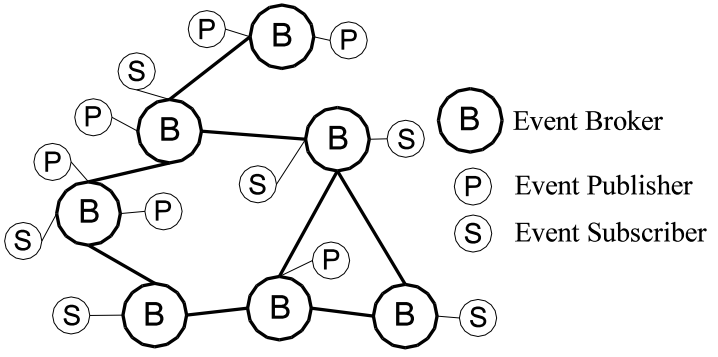
\includegraphics[scale=0.5]{afbeelding/pubsubArchi.png}}
\caption{Broker netwerk \citep{pietzuch2002hermes}}
\label{fig:pubsubArchi}
\end{figure}

Een naïeve aanpak, volgens \citet{carzaniga2001design}, is het gebruiken van één centrale server waar alle subscripties worden bijgehouden, waar alle events toekomen, waar de bestemming van het event beslist wordt en waar het event wordt doorgestuurd naar de gepaste subscribers.
Deze strategie is eenvoudig te implementeren maar deze werkt de schaalbaarheid tegen.
Dit was ook al duidelijk in Figuur~\ref{fig:pubsubArchi} waar verschillende ``Brokers'' aanwezig zijn.
Het is belangrijk om stil te staan bij enkele ontwerp beslissingen zodanig dat de service die in Figuur~\ref{fig:pubsubService} zichtbaar is, implementeerbaar is.

\begin{figure}[!ht]
\centering
\makebox[0pt]{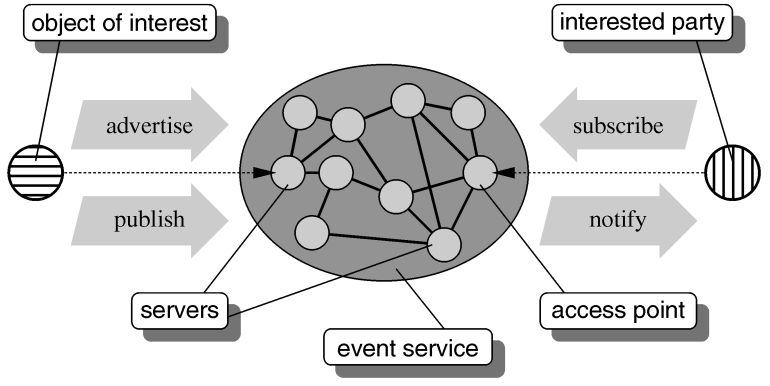
\includegraphics[scale=0.5]{afbeelding/pubsub.png}}
\caption{Publish/Subscribe service \citep{carzaniga2001design}}
\label{fig:pubsubService}
\end{figure}

Naast de architectuur is het belangrijk om te weten wat wordt verzonden en op welke manier.
\citet{carzaniga2001design} haalt een structuur aan waarin een event beschreven wordt als een set van attributen.
Ieder attribuut bestaat uit een type, naam en waarde.
De naam van een attribuut is een string en het type komt uit een set van primitieven die terug gevonden worden bij de meeste hedendaagse programmeertalen.
Een voorbeeld van zo'n event is terug te vinden in Figuur~\vref{fig:pubsubNot}

\begin{figure}[!ht]
\centering
\makebox[0pt]{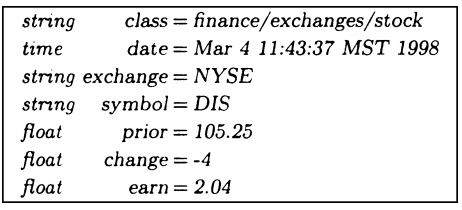
\includegraphics[scale=0.5]{afbeelding/pubsubNot.png}}
\caption{Publish/Subscribe Event \citep{carzaniga2001design}}
\label{fig:pubsubNot}
\end{figure}

\section{Technologieën voor software packaging}\label{sec:technologieen}
In de vorige secties werden oplossingen gezocht voor het verspreiden van software naar verschillende gebruikers.
Hierbij werd vooral rekening gehouden met op welke wijze de software verzonden word.
Er werd nagegaan of een oplossing zorgde voor een schaalbare architectuur die mogelijkheden biedt naar de toekomst toe.
Er werd zelfs gezocht naar een rampenplan dat gebruikt kan worden als er fouten optreden tijdens het installatieproces (Sectie~\vref{sec:rollback}.
In wat volgt wordt niet meer gekeken naar hoe de software bij de gebruiker raakt maar wat er bij de gebruiker raakt.

Implementaties in verschillende programmeertalen, verschillende data representatie formats of incompatibele runtime environments kunnen aan de basis liggen voor een lastige integratie van computerprogramma's.
Door gebruik te maken van additionele software, wordt het mogelijk om het gat tussen de verschillen te overbruggen  \citep{callahan1998software}.
Het Python testraamwerk is een verzameling van verschillende drivers en bibliotheken elk met een eigen implementatie.
Door additionele software toe te voegen is het mogelijk dat verschillende software ``pakketten'' op een gelijkaardige manier behandelt worden.
In wat volgt zullen verschillende technologieën en tools besproken worden die ervoor zorgen dat verschillende software ``pakketten'' een geheel vormen.
Dit geheel kan vervolgens verzonden worden naar de gebruikers waar de software geïnstalleerd moet worden.

Om de verschillende technologieën te vergelijken werd een algemeen testscenario uitgedacht.
Het scenario ziet er als volgt uit: er moet een geheel gemaakt worden waarmee twee verschillende pakketten (die drivers en bibliotheken moeten voorstellen) geïnstalleerd moeten worden.
Hierna werd er onderzocht hoe één van de twee pakketten geüpdatet kon worden.
Door de technologieën te onderwerpen aan een test, wordt het mogelijk om de voor- en nadelen van iedere technologie te achterhalen.
Hiernaast wordt het ook mogelijk om de technologieën te vergelijken aangezien zij eenzelfde functionaliteit moeten voorzien.

\begin{table}[]
\centering
\begin{tabular*}{\linewidth}{clll}
\hline
\multicolumn{4}{p{\linewidth}}{\centering \textbf{WiX Toolset}}                    \\ 
\multicolumn{2}{p{0.5\linewidth}}{\centering Pro} & \multicolumn{2}{p{0.5\linewidth}}{\centering Cons} \\ \hline
\multicolumn{2}{p{0.5\linewidth}}{Diepe integratie met Windows \par Mogelijkheid om externe executables te includeren}   & \multicolumn{2}{p{0.5\linewidth}}{XML structuren zorgt voor veel overhead \par Niet cross-platform}    \\ \hline
\multicolumn{4}{p{\linewidth}}{\centering \textbf{NSIS}}                           \\ 
\multicolumn{2}{p{0.5\linewidth}}{\centering Pro} & \multicolumn{2}{p{0.5\linewidth}}{\centering Cons} \\ \hline
\multicolumn{2}{p{0.5\linewidth}}{Scripting taal \par Verschillende plug-ins beschikbaar}   & \multicolumn{2}{p{0.5\linewidth}}{ Niet cross-platform \par Geen structuur voor packages}    \\ \hline
\multicolumn{4}{p{\linewidth}}{\centering \textbf{Chocolatey}}                     \\ 
\multicolumn{2}{p{0.5\linewidth}}{\centering Pro} & \multicolumn{2}{p{0.5\linewidth}}{\centering Cons} \\ \hline
\multicolumn{2}{p{0.5\linewidth}}{Volledige deployment infrastructuur al aanwezig}   & \multicolumn{2}{p{0.5\linewidth}}{Niet cross-platform \par Command-line tool}    \\ \hline
\multicolumn{4}{p{\linewidth}}{\centering \textbf{Qt Installer Framework}}         \\ 
\multicolumn{2}{p{0.5\linewidth}}{\centering Pro} & \multicolumn{2}{p{0.5\linewidth}}{\centering Cons} \\ \hline
\multicolumn{2}{p{0.5\linewidth}}{Cross-platform \par Mogelijkheid om externe executables te includeren}   & \multicolumn{2}{p{0.5\linewidth}}{XML structuren zorgt voor veel schrijfwerk \par Enkel Linux installer maken in Linux} \\ \hline
\end{tabular*}
\caption{Voor- en nadelen van de verschillende technologieën}
\label{tab:voorNadelen}
\end{table}

\subsubsection{WiX Toolset}
Windows installer XML Toolset is een set van build tools waarmee Windows Installer packages gemaakt worden van XML broncode.
De toolset is geschreven in C\# en heeft het .Net framework nodig om te kunnen functioneren.
Bron code wordt gecompileerd en vervolgens gelinkt om een executable te maken.
Met de toolset kunnen .msi installatie pakketten, .msm merge modules en .msp patches gecombineerd worden tot een Windows executabel.\citep{wixToolset}.

Aan deze technologie zijn verschillende voor- en nadelen verbonden (zie Tabel~\ref{tab:voorNadelen}).
Een fragment van de WiX toolset code is terug te vinden in Listing~\vref{list:wix}.
De WiX toolset maakt installer uitsluitend bedoelt voor de Windows installation engine.
Hierdoor worden verscheidene functionaliteiten eenvoudig te gebruiken, zoals het maken van uitzonderingen in de Windows Firewall.
Door gebruik te maken van de Windows installation engine is het niet mogelijk om de executabel te gebruiken in Linux omgevingen\footnote{Dit kan eventueel omzeilt worden door het gebruik te maken van software zoals Wine \citep{amstadt1994wine}. Als geen alternatieven aanwezig zijn, dan is deze strategie eventueel het overwegen waard.}.
WiX maakt gebruik van XML broncode om verschillende elementen te definiëren.
\citet{xmill} geeft al aan dat XML niet een van de meest efficiënte dataformaten is, maar het verhoogd de flexibiliteit wel.
Het creëren van een XML bestand met de hand is een langdradig en moeilijk werk.

\subsubsection{NSIS}
Nullsoft Scriptable Install System is een open source systeem waarmee Windows installers gemaakt kunnen worden.
Zoals de naam aangeeft, is NSIS script-based.
Hierdoor bevatten installers de nodige om verschillende installatie taken uit te voeren.
Door de grote gebruikersbasis is een grote hoeveelheid plug-ins en scripts beschikbaar.
Alle plug-ins en scripts kunnen op een eenvoudige manier aan een installer toegevoegd worden voor een verhoogde functionaliteit \citep{nsisMain}.

De voor- en nadelen verbonden aan NSIS zijn terug te vinden in Tabel~\ref{tab:voorNadelen}.
Met de scripting taal van NSIS is het mogelijk om eenvoudige installer te definiëren (een voorbeeld hiervan is terug te vinden in Listing~\vref{list:nsis}).
De scripting taal is intuïtiever te gebruiken in vergelijking met de XML bestanden van Wix Toolset.
Dankzij grote hoeveelheid aan plug-ins die aanwezig zijn, is het eenvoudig om een installer te creëren met verschillende functionaliteiten.
De gecreëerde installer is een Windows executabel en de opmerking gegeven bij de WiX Toolset is hier ook van toepassing.
Het feit dat NSIS bedoelt is om eenvoudige installers te maken zorgt ervoor dat het niet mogelijk is om aparte pakketten te definiëren.
Ieder pakket kan wel een eigen configuratie hebben maar dit wordt allemaal toegevoegd aan één script.
Bij een grote hoeveelheid aan pakketten leidt tot wanorde en is er geen globaal overzicht.
NSIS beidt ook geen mogelijkheden aan om geïnstalleerde software up te daten.
Om die eigenschappen toe te voegen moet er beroep gedaan worden op andere software.

\subsubsection{Chocolatey}
Volgens \citep{chocoAbout} is Chocolatey een package mangager voor Windows net zoals apt-get voor Linux is.
Het is ontworpen als een gedecentraliseerd framework met als doel het snel installeren van applicaties en tools.
Chocolatey werd gebouwd boven op de NuGet infrastructuur gecombineerd voor het verspreiden van de packages en gebruikt PowerShell voor een gepersonaliseerde installatie.

In Tabel~\ref{tab:voorNadelen} zijn de verschillende voor- en nadelen gekoppeld aan Chocolatey terug te vinden.
Het grootste voordeel dat bekomen wordt bij het gebruiken van een package manager is het al bestaan van een deployment infrastructuur. 
Na het installeren van Chocolatey op de client kunnen alle nodige packages voor het framework geïnstalleerd worden.
Hiernaast kunnen scripts gekoppeld worden aan iedere package zodanig dat een aangepaste installatie mogelijk is.
Net zoals apt-get voor Linux, is Chocolatey te gebruiken in de command-line.
Dit is vooral een nadeel naar gebruiksvriendelijkheid toe aangezien er vanuit wordt gegaan dat de gebruikers amper tot geen ervaring hebben met de command-line in Windows/Linux.
Het grootste nadeel aan deze technologie is, net zoals de vorige opties, het niet cross-platform zijn.

\subsubsection{Qt Installer Framework}
Het Qt Installer Framework biedt een set van tools aan voor het creëren van installers op verschillende platformen.
Aan de hand van een set van pagina's wordt de gebruiker door het installatie-, update- en verwijderproces.
Hierbij kunnen scripts gebruikt worden om het proces te vereenvoudigen \citep{qtDoc}.
Door een folder structuur op te bouwen zoals zichtbaar is in Figuur~\vref{fig:folder} kan het Qt installer framework een installer creëren die vervolgens op het doelsysteem uitgevoerd kan worden.

\begin{figure}[!ht]
\centering
\makebox[0pt]{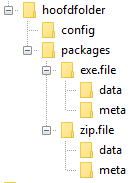
\includegraphics[scale=0.9]{afbeelding/folder.png}}
\caption{Folder structuur voor installer}
\label{fig:folder}
\end{figure}

De data folder van een pakket bevat alle nodige databestanden die moeten uitgevoerd worden (zoals een executable of een zip archief).
De meta folder bevat een beschrijving van het pakket (zie voorbeeld in Listing~\vref{list:qtpakket}).
Hiernaast is ook een installatiescript aanwezig dat uitgevoerd wordt tijdens de installatie van het pakket zelf (zie Listing~\vref{list:qtscript}).
Met de installer informatie uit de config folder (zie Listing~\vref{list:qtqtinstaller}) weet het Qt installer framework voldoende om een executable te produceren die alle pakketten installeert aan de hand van de opgegeven installatiescripts.
Op deze wijze is het mogelijk om verschillende pakketten te combineren tot één geheel en ondertussen toch ieder pakket apart te behandelen.

Aan deze technologie zijn verschillende plus- en minpunten verbonden.
Een vergelijking van de verschillende voor- en nadelen is terug te vinden in Tabel~\ref{tab:voorNadelen}.
Het grootste voordeel van het Qt Installer framework is het cross-platform zijn.
Hierdoor is het mogelijk om installers te maken voor zowel Windows als Linux.
Een nadeel dat hieraan verbonden is, is dat een Linux installer enkel kan gemaakt worden op in een Linux omgeving.
Het is niet mogelijk om een Linux installer te maken op een Windows systeem.
Hiernaast is het wel mogelijk om voor ieder pakket een aparte installatieprocedure te implementeren.

%%% TODO Schrijven over het gebruiken van Windows .exe in Linux? Bijvoorbeeld hoe Wine misschien een oplossing is?

%%% TODO Schrijven over de test setup voor de verschillende technologieën die gebruikt is tijdens de stage?
\chapter{Analyse en ontwerp}\label{sec:anaEnOntwerp}
\section{Inleiding}
Uit de probleemstelling werd het snel duidelijk dat het probleem omtrent het installeren en updaten van programma's complexer is dan op het eerste zicht lijkt.
In dit hoofdstuk zal het probleem verder geanalyseerd worden.
Aan de hand van deze bevindingen gaat een architectuur ontworpen of geselecteerd worden.
Deze vormen de basis voor de implementatie van de demo.

\section{Analyse}
Het probleem van Televic was het volgende:
Televic fabriceert producten die moeten voldoen aan strenge veiligheidsnormen.
Om hun producten hierop te kunnen testen heeft Televic een Python testraamwerk ontworpen waarmee het mogelijk wordt om de producten aan verschillende testscenario's te onderwerpen.
Dit testraamwerk maakt gebruik van een grote set aan drivers en bibliotheken om een correcte werking te garanderen.
Een direct gevolg hiervan is dat het installatieproces op een nieuwe testtoren veel tijd in beslag neemt en foutgevoelig is.
Het is belangrijk om rekening te houden met deze fouten en een rampenplan te voorzien.
Hiernaast groeit het aantal gebruikers van het testraamwerk continu samen met het aantal drivers, bibliotheken en programma's die verspreid moeten worden.
Verder dient elk nieuw toestel op het raamwerk ondersteund te worden waardoor er jaarlijks ettelijke releases van het raamwerk verspreid moeten worden.
Er moet dus een antwoord gegeven worden op de volgende vragen:
\begin{itemize}
\item Wat moet verzonden worden naar de gebruikers?
\item Hoe raakt de software van de producent bij de gebruiker?
\end{itemize}
Het doel is om een systeem te ontwikkelen dat Televic kan bijstaan bij het installatieproces en verspreidingsproces maar ook om een systeem te ontwikkelen dat kan blijven gebruikt worden in de toekomst.
Schaalbaarheid en flexibiliteit zijn hierbij zeer belangrijk.

%Packager
De probleemanalyse onthulde dus dat het probleem onder te verdelen is in verschillende deelproblemen (Wat wordt verzonden en hoe wordt dit aangepakt).
Het testraamwerk bestaat uit verschillende componenten, hieronder vallen de drivers en bibliotheken.
Elke component heeft een aparte installatiewijze en sommige componenten moeten voor andere geïnstalleerd worden.
Zo zal Python één van de eerste componenten zijn die geïnstalleerd moet worden.
Hiernaast moeten verscheidene componenten geconfigureerd tijdens het installatieproces aan de hand van een configuratiebestand.
Dit configuratiebestand is afhankelijk van testtoren waarop het testraamwerk op geïnstalleerd word.
Door gebruik te maken van additionele software worden verschillen in implementaties, door bijvoorbeeld verschillende programmeertalen, opgevangen.
Een deel van de applicatie zal dus bestaan uit deze additionele software die instaat voor het inpakken van de componenten: de \emph{packager}.
Hiervoor kan beroep gedaan worden op verscheidene technologieën, structuren en architecturen die besproken werden in Sectie~\ref{sec:technologieen}.
Door gebruik te maken van één van deze technologieën is geweten wat er wordt verzonden.

%Server
Naast de wat moet er ook geweten zijn hoe de software bij de gebruikers moet geraken.
Door dit proces te automatiseren, is het mogelijk om waardevolle informatie te verzamelen.
Met deze informatie kunnen rapporten gegeneerd worden over het deployment proces.
In Secties~\ref{sec:deployment} - \ref{sec:caseStudies} werden verschillende problemen maar ook oplossingen besproken die aan de basis liggen voor het ontwerp van dit onderdeel van de applicatie. 
In het vervolg van de thesis zal dit onderdeel (dat zal instaan voor het verspreiden van het testraamwerk maar ook voor de communicatie tussen de producten van het testraamwerk en de gebruikers) vermeld worden als de \emph{deployment server}.

%Environment
In Sectie~\vref{sec:softwareLevenscyclus} werd besproken welke problemen kunnen optreden tijdens het installatieproces.
Deze problemen moeten opgevangen worden om een schaalbare oplossing te bedenken voor Televic.
Om dit op te vangen, kan er gebruik gemaakt worden van één (of meerdere) strategieën die besproken werd in Sectie~\vref{sec:rollback}.
Dit onderdeel van de applicatie vooral aanwezig aan de client-side aangezien dat de plaats is waar het testraamwerk aanwezig zal zijn.
In de loop van de thesis zal naar dit onderdeel verwezen worden als de \emph{deployment environment}.

Na de probleemanalyse is het nu duidelijk dat het werk op te delen valt in drie grote componenten.
Deze drie onderdelen zullen de basis vormen voor de architectuur en zullen gebruikt worden als leidraad.
Het eerste onderdeel zal bestaan uit de packager met als doel het inpakken van de nodige drivers, bibliotheken, \ldots .
Naast de packager is er de deployment server instaat voor het verspreiden van de installers die de packager aflevert.
Aan de client-side zal de deployment environment aanwezig zijn waardoor installatie-complicaties vermindert worden door de installatie te isoleren.
Mocht een rollback nodig zijn, dan kan deze op een eenvoudige manier gebeuren.
In Figuur~\vref{fig:overzichtsDiagram} wordt de algemene structuur van de applicatie weergegeven.
Met behulp van deze basis is het mogelijk om een demo te produceren voor de finale verdediging.

\begin{figure}[!hbt]
\centering
  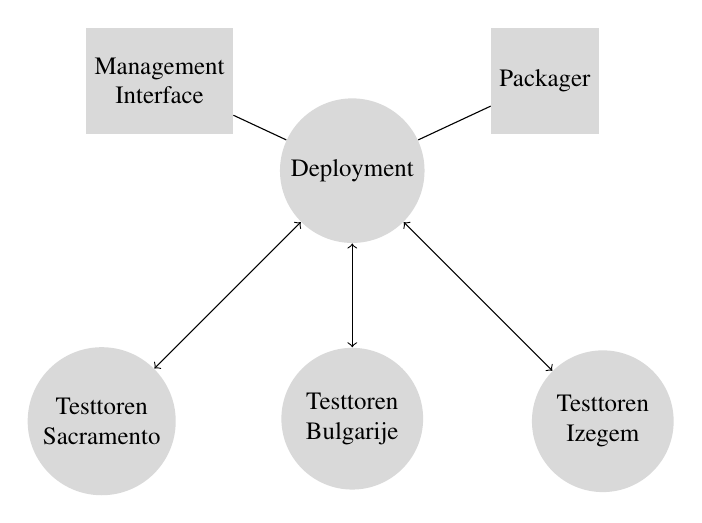
\begin{tikzpicture}[scale=.9, transform shape]
\tikzstyle{every node} = [circle, minimum size = 2cm, fill=gray!30]
\node (a) at (0, 0) {Deployment};
\node[shape = rectangle,minimum size = 1.5cm] (packager) at +(25: 3) {Packager};
\node[shape = rectangle,minimum size = 1.5cm, align=center] (logger) at +(155: 3) {Management\\ Interface};
\node[align=center] (b) at +(225: 5) {Testtoren\\ Sacramento};
\node[align=center] (c) at +(270: 3.5) {Testtoren\\ Bulgarije};
\node[align=center] (d) at +(315: 5) {Testtoren\\ Izegem};
\foreach \from/\to in {a/b, a/c, a/d}
\draw [<->] (\from) -- (\to);
\draw [-] (a) -- (packager);
\draw [-] (a) -- (logger);
\end{tikzpicture}
  \caption{Overzichtsdiagram van de algemene structuur}
  \label{fig:overzichtsDiagram}
\end{figure}


\section{Architectuur}

\subsection{Databank ontwerp}\label{sec:databank}
Eén van de problemen is de continue toename aan pakketten waar het framework gebruikt van maakt en het aantal gebruikers die het framework gebruiken.
Om dit probleem aan te pakken wordt een databank ontworpen voor het opslaan van alle cruciale data over zowel het installatieproces en als de gebruikers.
In overleg met Televic werd ervoor gekozen om MySQL te gebruiken als managementsysteem.
Het ontwerp van de databank is terug te vinden in Figuur~\ref{fig:databank}.

\begin{figure}[!ht]
\centering
\makebox[0pt]{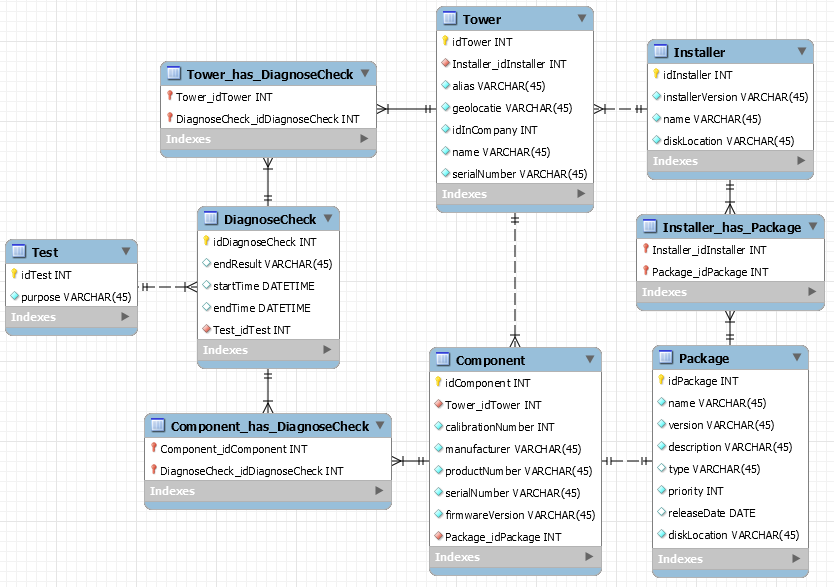
\includegraphics[scale=0.7]{afbeelding/databankOntwerp.png}}
\caption{Ontwerp van de databank}
\label{fig:databank}
\end{figure}

De tabellen tower en hardware\_component dienen om iedere gebruiker, typisch een testtoren of een laptop, te beschrijven.
Iedere toren heeft een ID, naam en serienummer.
De combinatie van deze drie waarden is uniek binnen het bedrijf en de combinatie kan gebruikt worden als identificatie binnen het systeem maar deze combinatie draagt geen betekenis voor een gebruiker.
Om dit op te vangen wordt aan iedere toren een alias gekoppeld waardoor de identificatie voor mensen vlotter kan verlopen.
Elke toren bestaat typisch uit verschillende hardwarecomponenten, zoals voedingen of netwerkkaarten, die nodig zijn om testen uit te voeren.
Iedere component is gemaakt door een bepaalde fabrikant en krijgt van de fabrikant een serienummer.
Vanuit het bedrijf wordt losstaand hiervan een nummer toegekend aan iedere component die gebruikt wordt om de calibratie instellingen te achterhalen.
Iedere hardwarecomponent gebruikt firmware om correct te functioneren.
Naast alle bovengenoemde informatie wordt ook de versie van de firmware opgeslagen.
Door het opslaan van al deze informatie wordt het mogelijk om:
\begin{enumerate}
\item Torens van elkaar te onderscheiden
\item Hardware componenten te koppelen aan torens
\item Firmware versies te koppelen aan hardware componenten
\end{enumerate}

Naast informatie over de gebruikers wordt ook informatie over de verschillende installers en pakketten bijgehouden.
Een installer bestaat uit een combinatie van verschillende software pakketten.
Bij deze pakketten moet één pakket aanwezig zijn dat het Python testraamwerk bevat.
Hiernaast zijn verschillende andere pakketten aanwezig voor drivers.
In Figuur~\vref{fig:installerStructuur} is een voorbeeld zichtbaar van een installer die bestaat uit drie verschillende pakketten.
Eén pakket wordt gebruikt door het testraamwerk en de twee anderen voor drivers die nodig zijn om het testraamwerk correct te laten functioneren.
Iedere toren wordt gekoppeld aan één installer en zo aan één testraamwerk.
Hiernaast is het mogelijk om pakketten te koppelen aan hardware componenten.
Zo kan een driver voor een voeding gekoppeld worden aan de entry van de voeding die aanwezig is in de hardware\_component tabel.
Op deze wijze worden de hardware-software afhankelijkheden bijgehouden.
Van ieder pakket wordt bijgehouden welk type pakket het is (een executabel, zip bestand, \ldots), de prioriteit voor de installatievolgorde, een korte beschrijving en de release datum.
Naast al deze informatie wordt er ook bijgehouden welke pakketten afhankelijk zijn van elkaar.
Een voorbeeld is hiervan is een testraamwerkpakket en een pakket waarmee Python geïnstalleerd wordt.
Het testraamwerk is afhankelijk van Python om correct te functioneren.
Zo worden de verschillende software-software afhankelijkheden bijgehouden.
Voordat een installer gemaakt wordt, die een testraamwerkpakket bevat, kan gecontroleerd worden dat ook het Python-installatiepakket aanwezig is.

\begin{figure}[!ht]
\centering
\makebox[0pt]{\includegraphics[scale=0.4]{afbeelding/installerStructuur.png}}
\caption{Structuur van een installer bestaande uit drie pakketten}
\label{fig:installerStructuur}
\end{figure}

Verder zijn er enkele tabellen aanwezig voor het ondersteunen van testen.
Tijdens en na het installatieproces moet het mogelijk zijn om testen uit te voeren.
Dankzij deze testen is het duidelijk of een bepaald pakket correct functioneert en op het einde van het installatieproces kan gecontroleerd worden of het volledige testraamwerk in zijn geheel functioneert.
Doordat er een link wordt bijgehouden tussen een hardware component en een pakket, is het mogelijk om hieruit waardevolle informatie te halen.
Zo kan bijvoorbeeld een verband gelegd worden tussen een bepaalde versie van een driver en de firmware die aanwezig is in een hardware component.
Deze informatie kan gebruikt worden om problemen in testtorens te vermijden.

\subsection{Packager}
De architectuur van de packager wordt gebaseerd op de architectuur en structuur van het Qt installer framework.
Er wordt een installer geproduceerd die bestaat uit verschillende pakketten die elk instaan voor het installeren van een software component.
Voor iedere installer wordt een aparte folder structuur aangemaakt die zichtbaar is in Figuur~\vref{fig:installerStructuur}.
In de config folder van de installer worden alle globale scripts en beschrijvingsbestanden bijgehouden.
Verder bevat de installer subtrees voor ieder pakket.
Een pakket bestaat vervolgens uit een data, include en meta folder.
De data folder wordt gebruikt om de effectieve driver/bibliotheek in op te slaan.
Hiernaast is een include folder aanwezig waarin verschillende afzonderlijke scripts toegevoegd kunnen worden.
Op deze manier kunnen willekeurige scripts (bijvoorbeeld een script die de firewall instellingen aanpast) rap toegevoegd worden aan een pakket.
Als laatste bevat de meta folder alle meta-data horende het pakket.
Dit omvat onder andere een script die gebruikt wordt om te testen of het pakket wel correct functioneert maar ook een beschrijving van het pakket zelf.

%het zorgt voor een beter bereik van de verschillende packages -> kunnen test tussendoor uitvoeren
Door zelf een packager te produceren, is het mogelijk om iedere stap in het deployment proces te personaliseren.
Op deze manier kan na het installeren van een pakket een zo optimaal mogelijke afhandeling plaats vinden.
Zo kunnen testen op ieder moment in het installatieproces toegevoegd worden, een handeling die met het Qt installer framework ook mogelijk is maar dit is moeilijker te realiseren.
%geen gedoe met docker
Doordat een gepersonaliseerde packager wordt ontworpen, worden problemen met Docker vermeden.
Verder wordt besproken hoe Docker gebruikt wordt in de deployment environment om verscheidene problemen die gerelateerd zijn aan het installatieproces op te vangen.
De Docker omgeving, zoals reeds vermeld in Sectie~\vref{sec:docker}, maakt gebruikt van LXC.
Het besturingssysteem van de containers is hierdoor Linux.
Windows gebruiken als besturingssysteem voor de containers is mogelijk in Docker is mogelijk maar deze optie staat nog altijd in beta schoenen.
Mocht het Qt installer framework gebruikt worden als packager, dan moet het besturingssysteem van de server ook Linux zijn.
Door ervoor te kiezen om zelf een packager te produceren, kan voor een cross-platform oplossing gezocht worden en kan de integratie van Docker vlotter verlopen.
Op deze manier wordt er een abstractie gemaakt van het besturingssysteem van zowel de server als client.

\subsection{Deployment server}
Het centrale systeem in de architectuur is de deployment server.
Zoals reeds uitgelegd zal dit onderdeel instaan voor het verspreiden van de verschillende installers en functioneren als een verzamelcenter voor alle informatie.
De architectuur van de deployment server wordt gebaseerd op de software dock architectuur die besproken werd in Sectie~\vref{sec:softwareDock} en is terug te vinden in Figuur~\vref{fig:softwareDockAangepast}.
De software dock architectuur bestaat uit 4 grote componenten, namelijk het release dock, field dock, event service en de agenten.

\begin{figure}[!ht]
\centering
\makebox[0pt]{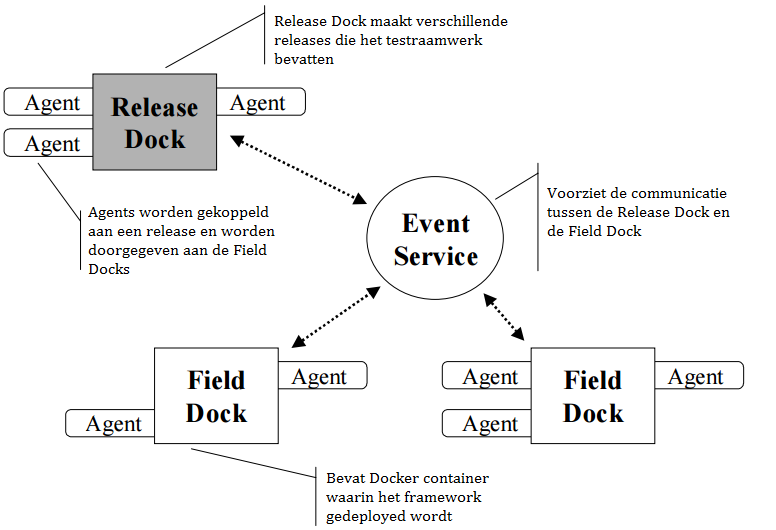
\includegraphics[scale=0.5]{afbeelding/softwareDockAangepast.png}}
\caption{Software Dock Architectuur \citep{hall1999cooperative}}
\label{fig:softwareDockAangepast}
\end{figure}

\paragraph{Release Dock}
Het release dock bevindt zich aan de serverzijde en bevat de code voor zowel de packager als de monitor van de clients.
Met hulp van de packager worden de verschillende installers geproduceerd.
Naast het produceren van installers zal het release dock instaan voor het monitoren van de field docks.
Hier wordt vooral gebruik gemaakt van de verschillende resultaten van de test die uitgevoerd worden tijdens het installatieproces.
Op de manier wordt achterhaalt welke installer geïnstalleerd werd op een field dock en welke fouten eventueel optraden tijdens het installatieproces.

\paragraph{Event Service}
Nevens de verschillende docks beschrijft de software dock architectuur een Event Service.
Deze staat in voor het afhandelen van de communicatie tussen de verschillende docks.
Om dit te implementeren, wordt er beroep gedaan op Sectie~\vref{sec:event}.
Er worden evenwel enkele kleine aanpassingen gemaakt.
De broker worden verschillende lijsten bijgehouden voor ieder type van bericht dat mogelijk is.
Bij het toekomen van een subscribe/unsubscribe bericht, zal de broker de nodige lijsten aanpassen zodat de zender van het bericht wordt toegevoegd of verwijderd.
Berichten in het netwerk zullen bestaan uit een set van attributen en waarden in een JSON formaat.
Het uiterlijk van zo'n bericht is gelijkaardig als het uiterlijk van een bericht in Figuur~\vref{fig:pubsubNot}.
In Listing~\vref{list:bericht} wordt een voorbeeld van een bericht weergegeven.
Ieder bericht heeft dezelfde set aan attributen die elk een eigen functie hebben:
\begin{itemize}
\item \emph{Timestamp}: ieder bericht zal op het moment van de creatie een timestamp krijgen.
De timestamp wordt uitgedrukt in seconden sinds epoch.
Op deze wijze wordt eenzelfde referentie punt gebruikt en is het mogelijk om de creatie van berichten in de tijd te ordenen.
\item \emph{Type}: ieder bericht hoort toe aan een bepaald type.
De verschillende types van berichten zijn: subscribe, unsubscribe, new, change, rapport, update, release.
Afhankelijk van het type bericht dat toekomt, bij zowel de broker als een dock, zal een andere actie ondernomen worden.
De eerste twee types zijn uitsluitend bedoelt voor de broker.
De volgende drie voor een release dock en de laatste twee voor de field docks.
\item \emph{ID}: naast een timestamp wordt aan ieder bericht een id meegegeven. 
Dit attribuut wordt meegegeven zodanig dat de field docks kunnen achterhalen of zij achterlopen op berichten.
\item \emph{Data}: Dit is het meest flexibele attribuut. 
Hier wordt de data meegegeven die hoort bij het bericht.
Als het type van een bericht ``subscribe'' is, dan zit in het data veld een lijst met alle types waarvoor de gebruiker zich voor wilt inschrijven.
\item \emph{Sender}: Het laatste attribuut dat wordt meegegeven is de zender van het bericht.
De broker moet bij een subscribe bericht kunnen achterhalen wie de zender is.
Op die manier weet de broker wie moet worden toegevoegd aan de nodige lijsten.
\end{itemize}

\begin{minipage}{\linewidth}
\begin{center}
\begin{lstlisting}[caption={Format voor een bericht},label={list:bericht}, xleftmargin=.3\textwidth]
{
 'timestamp': 1491982212.555,
 'type': 'subscribe',
 'id': 0,
 'data': {
   'type': [
     'new',
     'change',
     'rapport'
   ]
 },
 'sender': 'localhost'
}
\end{lstlisting}
\end{center}
\end{minipage}

\paragraph{Agenten}
%%schrijven over hoe de agenten werken en hoe ze gaan werken volgens de handelingen van ORYA
Naast de docks beschrijft de software dock architectuur ook agenten.
Deze staan in voor het uitvoeren van allerlei deployment gerelateerde handelingen.
Iedere agent is gekoppeld aan één stap uit de software levenscyclus die besproken werd in Sectie~\vref{sec:softwareLevenscyclus}.
Hiernaast zal aan iedere installer afkomstig van het release dock een subset van alle agenten toegevoegd en verscheept worden naar het field dock.
Op deze manier is het mogelijk om iedere stap in de levenscyclus van de installer te personaliseren.
Ieder agent zal een bepaalde set van handelingen uitvoeren die overeenkomt met een deployment proces die besproken werd in de ORYA case studie in Sectie~\vref{sec:ORYA}.
Net zoals bij ORYA wordt ieder deployment proces beschreven aan de hand van andere deployment processen en basis activiteiten.
Een voorbeeld:
Tijdens de creatie van een installer wordt een agent voorzien die instaat voor het installatieproces.
De agent wordt samen met de installer verscheept naar het field dock waarna de agent op het gepaste moment in actie schiet.
De agent begint met het hernoemen van de oude Docker container met daarin de vorige versie van een installer.
Hierna wordt een nieuwe container aangemaakt waarin de nieuwe installer wordt losgelaten.
Vervolgens zal de agent de installatie aanvangen en zullen de scripts horende bij de pakketten uitgevoerd worden in de container.
Zoals reeds werd aangegeven, zijn de handelingen van een agent gebaseerd op het model van ORYA.
Zo wordt het creëren van een nieuwe container in de installatie agent wordt gezien als zo'n basis activiteit.
In Bijlage~\vref{sec:flowcharts} zijn verschillende flowcharts terug te vinden die horen bij enkele types van agenten.
Door agenten te gebruiken, een strategie die ook gezien werd in de Atlas case studie in Sectie~\vref{sec:ATLAS}, wordt het mogelijk om alle stappen in de software levenscyclus uniek te behandelen.
Hiernaast kan bij iedere installer een andere set van agenten geassocieerd worden waardoor iedere installer verder gepersonaliseerd kan worden.

\subsection{Deployment environment}
De deployment environment komt overeen met de field dock in de software dock architectuur.
In de omgeving gaat de installer, afkomstig van de packager, uitgevoerd worden zodanig dat het test framework geïnstalleerd wordt.
Aan dit proces zijn de verschillende problemen verbonden die besproken werden in Sectie~\vref{sec:softwareLevenscyclus}.
Om de verschillende deployment problemen te vermijden en om ervoor te zorgen dat geen uitgebreide rollback strategieën nodig zijn, wordt een geïsoleerde omgeving voorzien waarin de software geïnstalleerd wordt. 
Dit wordt gerealiseerd aan de hand van virtualisatie technieken, meer bepaald aan de hand van Docker.
Docker wordt verkozen boven een gewone virtuele machine omdat het uitvoeren van handelingen (zoals opstarten, stoppen, \ldots) op een container minder resources en tijd vraagt in vergelijking met een virtuele machine.
Doordat een virtualisatie techniek wordt gebruikt, wordt het zeer eenvoudig om problemen tijdens de verschillende processen op te vangen.
In Figuur~\vref{fig:flow:install} en Figuur~\vref{fig:flow:rollback} is het duidelijk dat, door het gebruik van Docker, het rollback proces zeer eenvoudig is.
Figuur~\vref{fig:fieldDock} geeft weer op welke manier de agenten met de containers gaan communiceren en geeft ook weer hoe Docker wordt geïntegreerd in het geheel.

\begin{figure}[!ht]
\centering
\makebox[0pt]{\includegraphics[scale=0.5]{afbeelding/fieldDock.png}}
\caption{Structuur van een field dock}
\label{fig:fieldDock}
\end{figure}

De volledige architectuur wordt weergegeven in Figuur~\vref{fig:architectuur}.
In de figuur worden de verschillende docks afgebeeld samen met zowel Docker als de packager.
Met deze architectuur is het mogelijk om aan de slag te gaan en een goede oplossing te vinden voor het probleem van Televic.

\begin{figure}[!ht]
\centering
\makebox[0pt]{\includegraphics[scale=0.5]{afbeelding/architectuur.png}}
\caption{Architectuur van het prototype}
\label{fig:architectuur}
\end{figure}

\chapter{Implementatie}
\section{Inleiding}
Na de literatuurstudie en de ontwerpfase, moet het ontwerp dat besproken werd in het vorige hoofdstuk geïmplementeerd worden.
Als programmeertaal werd Python gekozen.
In het bedrijf is een zeker kennis van Python aanwezig waardoor de overname vlotter zal verlopen.
Het doel is om een programma te ontwikkelen dat de belangrijkste functies omvat en dat gemakkelijk uitgebreid kan worden.
In de komende secties worden de verschillende implementatie beslissingen toegelicht en wordt de geschreven code toegelicht.
In wat volgt, zullen de server-side en client-side van elkaar gescheiden worden en afzonderlijk besproken worden.

\section{Server-side}
Zoals werd aangegeven in Hoofdstuk~\ref{sec:initServer} bestaat het opstarten van een server uit het creëren van een ReleaseDock object gevolgd door het creëren van een Broker object.
Vervolgens gaat het release dock zich inschrijven voor de nodige berichten (zie Figuur~\vref{fig:seqStartServer}).

\begin{figure}[!ht]
\centering
\makebox[0pt]{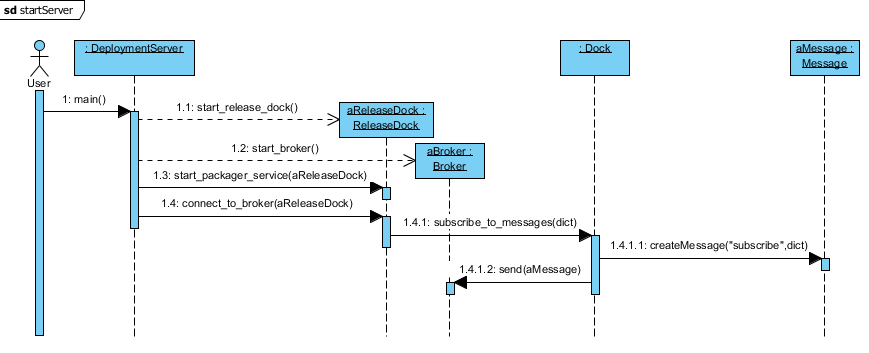
\includegraphics[width=\textwidth]{afbeelding/seqStartServer.png}}
\caption{Sequentie diagram voor het opstarten van een server}
\label{fig:seqStartServer}
\end{figure}

Bij het opstarten van de docks moeten verschillende parameters meegegeven worden.
Listing~\ref{list:startServer} geeft weer welke parameter ingevuld moeten worden voor een correcte functionaliteit.
De broker interface en port worden gebruikt door de Broker om een socket te openen maar ook door ReleaseDock om te connecteren met de broker.
De release\_dock interface en port zijn bedoelt voor in de ReleaseDock een poort te openen waar de Broker berichten naar kan verzenden.
Als laatste moeten de release interface en port gespecificeerd worden.
Met deze variabelen wordt een socket geopend die gebruikt wordt door het FieldDock om een installer op te halen\footnote{Het ophalen van een installer is het enige moment waarop een FieldDock direct contact opneemt met een ReleaseDock}.			

\begin{minipage}{\linewidth}
\begin{center}
%\lstset{language=Python}
\begin{lstlisting}[caption={Parameters voor server en broker},label={list:startServer}]
    broker_interface = "10.129.58.139"
    broker_port = 12347
    release_dock_interface = "10.129.58.139"
    release_dock_port = 12345
    release_interface = "10.129.58.139"
    release_port = 12346
\end{lstlisting}
\end{center}
\end{minipage}

\paragraph{Initialisatie} 
De server package bevat alle logica die hoort bij het release dock als bij de broker, maar bevat ook enkele modules die gebruikt worden om de realiteit af te beelden.
De flow van de applicatie begint met het opstarten van de deployment\_server module.
Deze module zal een release dock, een broker en een packager opstarten.
Vervolgens wordt het release dock gesubscribed voor de berichten van het type new, change en rapport.
Nadat de nodige services zijn opgestart, is het release dock klaar voor het afhandelen van alle nodige taken zoals het afhandelen van binnenkomende berichten.

Zowel het release dock als de broker erven eigenschappen van de klasse Dock.
Dit is zichtbaar in Figuur~\vref{fig:classDock}.
Aangezien alle docks en de broker dezelfde functionaliteiten moeten hebben (openen van een socket, luisteren voor data op de socket, versturen van berichten en afhandelen van berichten), is het eenvoudig om deze functionaliteiten in de superklasse te steken.
Voor de verschillende threads die gebruikt worden voor het luisteren naar nieuwe informatie maar ook voor het afhandelen Om de verscheidene threads te implementeren, werd altijd gebruik gemaakt van methodes die blocking zijn.
Op deze manier wordt ervoor gezorgd dat threads geen onnodige resources gebruiken.
Een soortgelijke strategie wordt toegepast voor de agenten aangezien elk type van agent een actie moet kunnen uitvoeren.
De nodige methodes worden vervolgens ingevuld in de subklasse. 

\begin{figure}[!ht]
\centering
\makebox[0pt]{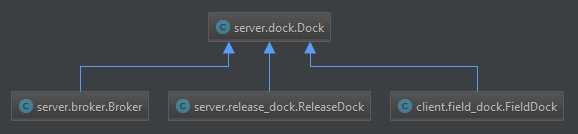
\includegraphics[scale=0.7]{afbeelding/classDock.png}}
\caption{Klassendiagram van Dock}
\label{fig:classDock}
\end{figure}

\paragraph{Grafische User Interfaces}
Het is ook mogelijk om de Grafische User Interface (GUI) op te starten door middel van de ``Enter'' toets.
Vanuit de GUI is het mogelijk om de verschillende clients te controleren en is het mogelijk om nieuwe installers te creëren.
De GUI werd gemaakt met de Python bibliotheek wxPython\footnote{\url{https://wxpython.org/}} en met de hulp van wxFormBuilder\footnote{\url{https://github.com/wxFormBuilder/wxFormBuilder}} werd basis code gegenereerd.
De nodige methodes werden vervolgens overschreven in de module overview\_impl.
Via deze methode wordt een gelijkaardig resultaat behaald voor het maken van de GUI voor de installer creatie.

\paragraph{Berichten versturen}
Bij het versturen van een bericht moet eerst een object aangemaakt worden van de Message klasse.
Vervolgens wordt de inhoud toegevoegd aan het bericht en kan het verzonden worden naar de broker.
In de broker wordt gecontroleerd welk type bericht het is om het dan vervolgens door te sturen naar alle doelen die in de gepaste list zitten.
Voordat het bericht wordt doorgestuurd wordt het eerst ingepakt in een ander bericht met als type notificatie.
Zo weet de ontvanger dat het bericht afkomstig is van de broker en is weet de ontvanger dat het data veld het doorgestuurde bericht bevat.
Deze kan vervolgens uitgepakt worden.
Afhankelijk van het type van het doorgestuurde bericht zal de correcte methode opgeroepen worden.

\paragraph{Installer creatie}
In de overzicht GUI is het mogelijk om een nieuwe installer te maken.
Met behulp van de aparte GUI, die geïmplementeerd wordt door de module release\_creator\_impl, is het mogelijk om een installer te definiëren.
Tijdens het samenstellen van de installer kunnen verscheidene nieuwe pakketten aangemaakt worden door de bovenste velden meermaals in te vullen.
Hierbij is het belangrijk om te weten dat een folder moet geselecteerd worden als bestandslocatie.
Alle bestanden aanwezig in de geselecteerde folder worden tijdens de creatie verplaatst naar de correcte locatie.
Bij het invullen van de gegevens van de installer moet ook een folder geselecteerd worden waarin de installer moet terecht komen.

Bij het indienen van de gegevens van de installer zelf worden de nodige handelingen uitgevoerd om een correcte installer te produceren.
Eerst worden de pakketten en installer toegevoegd aan de databank.
Vervolgens wordt de nodige folder structuur opgebouwd zoals aangegeven werd in Figuur~\vref{fig:installerStructuur}.
In de config folder wordt een leeg Dockerfile en een metadata bestand met daarin de volledige beschrijving van de installer.

Van zodra in de overview GUI het release signaal gegeven wordt, schiet het tweede deel van het release proces in werking.
Een install agent wordt aangemaakt en wordt toegevoegd aan de lijst van agenten horende bij de installer.
De folder structuur uit het eerste deel wordt gezipt zodanig dat minder data verzonden moet worden.
Als laatste deel van wordt een ``release'' bericht aangemaakt en verzonden naar de broker.
Deze schiet vervolgens in gang en stuurt het bericht door naar de nodige field docks.

\paragraph{Client monitoring}
In de applicatie is het mogelijk om in een beperkte manier de clients te controleren.
De overview GUI bevat een tabel met de verschillende clients die aanwezig zijn in de databank.
Met hulp van de mysql.connector module van Python lukt het om de databank te ondervragen.
Alle gegevens over de torens wordt opgevraagd en vervolgens worden er Tower objecten van gemaakt.
Hierna wordt gecontroleerd of op de toren een installer aanwezig is.
Mocht dit zo zijn, worden de gegevens over deze installer uit de databank gehaald.
Op deze manier kan nagekeken worden welke installer aanwezig is en kan dit worden weergegeven in de GUI.

\section{Client-side}
\paragraph{Initialisatie}
Aan de client-side wordt een gelijkaardige werkwijze gebruikt als bij de server-side.
De module deployment\_client zal een field dock object aanmaken en de nodige services aanpassen.
Tijdens het eerste gebruik van de code wordt een controle uitgevoerd waarmee gecontroleerd wordt of de description\_file aanwezig is.
Dit bestand bevat de volledige beschrijving van de testtoren met alle verschillende hardware componenten.
Vervolgens gaat het field dock zich subscriben voor de nodige berichten bij de broker.
Als beide stappen zijn afgelopen, wordt de Grafische User Interface opgestart en is het systeem klaar om gebruikt te worden.

\paragraph{Eerste gebruik}
Bij het eerste gebruik van de applicatie is de description\_file nog niet aanwezig.
Er is dan nog geen beschrijving van de gebruiker aanwezig aan zowel de client- als server-side.
Om dit aan te pakken, wordt een GUI opgestart waarmee het mogelijk is om het volledige systeem te beschrijven.
Na het invullen van de nodige informatie en het indienen van alle gegevens, wordt de description\_file aangemaakt.
Een ``new'' bericht wordt gefabriceerd met in het data veld de volledige beschrijving van het systeem.
Dit bericht wordt verzonden naar de broker en de broker stuurt het bericht door naar iedereen die gesubscribed is voor de ``new'' berichten.
Het bericht komt toe bij het release dock.
Het bericht wordt uitgepakt, omgevormd naar een Tower object en vervolgens toegevoegd aan de databank.

\paragraph{Installatieproces}
Van zodra een ``release'' bericht binnen komt bij het field dock schiet deze in gang om het installatieproces op poten te zetten.

Dill\footnote{\url{https://pypi.python.org/pypi/dill}} wordt gebruikt om de agent objecten te serialiseren voor ze verzonden worden naar het field dock.

De eerste actie die de install agent gaat ondernemen is het uitpakken van het zip bestand.
Met de Dockerfile uit de installer en de docker-py\footnote{\url{https://docker-py.readthedocs.io/en/stable/}} module wordt een Docker image aangemaakt die de basis zal vormen voor de container.
Voor de presentatie werd een image aangemaakt voor een Linux container waarin Python en wxPython op voorhand waren geïnstalleerd.
Vervolgens wordt een container gecreëerd met als naam ``fieldcontainer''.
Dit is de hoofdcontainer die altijd de laatst werkende versie van het framework zal bevatten.
Tijdens de creatie werden de nodige parameters doorgegeven om Grafische User Interfaces van de container op te kunnen starten.
Om dit mogelijk te maken, is het nodig om aan X11 forwarding te doen.
Belangrijk hierbij is dat op de host computer een X11 server moet draaien voordat dit kan plaats vinden.
Voor de demonstratie werd Cygwin\footnote{\url{https://www.cygwin.com/}} gebruikt om de X11 server op te starten en de correcte omgeving te generen\footnote{De tutorial \url{https://manomarks.net/2015/12/03/docker-gui-windows.html} werd hiervoor gevolgd}.
Hierna wordt het metadata bestand gelezen en gebruikt om de installatievolgorde van de pakketten te achterhalen.
Elk pakket wordt in de container gekopieerd en het installatie script wordt uitgevoerd.
Vervolgens gaat, met hulp van het test script, nagegaan worden of het installatieproces correct verlopen is.
De output van het script wordt gecontroleerd.
Als de uitgangsstatus begint met 0 wordt de test gezien als geslaagd.
Van zodra dit niet het geval is, wordt de container gemerkt als slecht en zal deze op het einde van het installatieproces in quarantaine geplaatst worden.
De container wordt niet verwijdert. 
Er werd voor deze strategie gekozen aangezien het mogelijk dat het test script slecht geschreven is.
Het framework is dan correct geïnstalleerd maar wordt door de test toch gezien als foutief.
Door de container in quarantaine te plaatsen blijft het mogelijk om achteraf test uit te voeren.
Vervolgens wordt een rapport aangemaakt met daarin het resultaat van de test, de begin- en eindtijd.
Het rapport wordt toegevoegd aan een bericht en wordt verzonden naar de broker die het doorstuurt.

\paragraph{Framework opstarten}
Na het opstarten van alle services verschijnt de Grafische User Interface van de client.
Van hieruit is het mogelijk om het pakket dat gemarkeerd staat als framework te openen.
De ``fieldcontainer'' wordt opgestart en het start script wordt uitgevoerd waardoor het framework zal opstarten.
\chapter{Evaluatie}
Na de ontwerp- en implementatiefase was het tijd om de gecreëerde applicatie te beoordelen en testen.
In het komende hoofdstuk is het dan ook de bedoeling om de applicatie te onderwerpen aan verschillende tests die enkele aspecten in de applicatie gaan testen.
Hierbij is het de bedoeling om te achterhalen wat wel en niet mogelijk is met de huidige versie van de applicatie.
Na het testen van de applicatie, wordt nagedacht voor mogelijke uitbreidingen voor de applicatie.

\section{Testen}
%%% TODO testen
\subsection{Cross-platform host}
\paragraph{Doel}
Het doel van deze test is het uittesten hoeverre de geschreven applicatie uitvoerbaar is op verschillende besturingssystemen.
De applicatie zelf is volledig geschreven in Python met modules die cross-platform zijn.

\paragraph{Scenario}
Om uit te testen of de applicatie cross-platform is, wordt een virtuele machine aangemaakt met de nodige programma's.
Als guest-besturingssysteem voor deze virtuele machine, wordt Linux Mint gekozen. 
Docker, Mysql workbench en wxPython worden geïnstalleerd en met hulp van pip worden de docker-py en dill modules aan python toegevoegd waardoor het systeem klaar is om getest te worden.
De databank werd aangemaakt en de code werd overgebracht naar de virtuele machine.

Tijdens de test is het de bedoeling om alle functionaliteiten van de applicatie uit te testen.
De verschillende docks moeten correct subscriben bij de broker en de nieuwe field dock moet zonder fouten worden toegevoegd aan de databank.
Vervolgens wordt getest of een installer kan aangemaakt worden, verscheept worden naar de field dock en geïnstalleerd kan worden.
Er wordt een installer aangemaakt die bestaat uit 3 verschillende pakketten: één framework pakket, één optioneel pakket en één niet-optioneel pakket.
De twee niet-framework pakketten bevatten een eenvoudig script die output genereert.
Het framework pakket bevat een Grafische User Interface gemaakt met wxPython.

De test is geslaagd als alle verschillende handelingen in de goede volgorde overlopen, ondertussen geen fouten optreden en op het einde het framework opgestart kan worden.

\paragraph{Uitvoering}


\subsection{Cross-platform containers}
\paragraph{Doel}
Naast het controleren of de applicatie zelf cross-platform is, is het belangrijk om te achterhalen of de applicatie om kan met Windows containers.
Het doel van deze test is dan ook om een installer te creëren specifiek bedoelt voor deze Windows containers.

\paragraph{Scenario}
Om gebruik te kunnen maken van Windows containers, moeten enkele vereisten voltooid worden.
Met hulp van \citet{windowsContainers} is het mogelijk om een field dock op te zetten die om kan gaan met de Windows containers.
De testomgeving bestaat, naast de enkele field dock, verder nog uit één release dock.
Deze wordt gebruikt om een installer te creëren die bestaat uit alle nodige pakketten om het Python testraamwerk werkende te krijgen.
Het framework pakket zal dan ook bestaan uit het daadwerkelijke testraamwerk.
Op deze wijze is het mogelijk voor Televic om te achterhalen welke stappen allemaal gezet zijn en welke nog moeten gezet worden om de applicatie zo snel mogelijk in gebruik te nemen.

\paragraph{Uitvoering}

\subsection{Meerdere clients}
\paragraph{Doel}
Voor deze test is het de bedoeling om te achterhalen of de applicatie meerdere clients kan ondersteunen.
Het doel is dan ook een omgeving op te zetten waarin verschillende clients aanwezig zijn.

\paragraph{Scenario}
De omgeving die gebruikt gaat worden bestaat uit één laptop die zowel gebruikt wordt als release dock en als field dock en twee andere computers die gebruikt worden als field docks.
Op de ieder computer is Docker, Python, wxPython, docker-py en dill aanwezig zodat de geschreven code bruikbaar is.

Tijdens de test wordt op één release dock een installer aangemaakt en klaargemaakt voor release.
De installer bestaat uit 2 verschillende pakketten: één framework pakket en één optioneel pakket.
Beide pakketten zullen bestaan uit enkele scripts die output zullen generen wanneer deze worden uitgevoerd.
Naast de release dock zullen 3 field docks toegevoegd worden aan het netwerk.

Om een geslaagde test te verkrijgen, moet de installer bij alle field docks toekomen en correct geïnstalleerd worden.
Dit moet op het einde van het proces zichtbaar zijn in zowel het overzicht op de release dock als in de databank.

\paragraph{Uitvoering}
Na het instellen van de nodige parameters, was het tijd om de nodige systemen op te starten.
Het duurde dan ook niet lang om drie torens te beschrijven die elk bestaan uit één hardware component.
Deze opstellingen werden vervolgens naar het release dock gestuurd en opgeslagen in de databank.

De volgende stap bestaat uit het beschrijven van een simpele installer bestaande uit twee pakketten en deze klaar te maken voor release.


\subsection{Meerdere servers}
\paragraph{Doel}
Een volgende test bestaat uit het testen van de functionaliteiten als meerdere servers aanwezig zijn.
Het doel van de test is te achterhalen wat er gebeurd als meerdere servers aanwezig zijn.

\paragraph{Scenario}
Na het testen of het mogelijk is om meerdere clients te ondersteunen, wordt nu getest of meerdere servers ondersteunt wordt.
Dit gebeurt wederom aan de hand van een virtuele machine met Windows 10.
Iedere virtuele machine bevat de server code samen met een databank om alle gegevens in op te slaan.

Gedurende de test worden 3 release docks aangemaakt en één field dock.
In het eerste deel van de test zal iedere release dock apart een installer creëren en deployen.
De installers zullen bestaan uit één pakket, namelijk een framework pakket.
Het pakket bevat een simpel script dat uitgevoerd wordt.
Voor ieder release dock zal dit script lichtjes verschillen.
Het tweede deel van de test bestaat uit het releasen van 3 verschillende installers op eenzelfde moment.
%%% TODO hier nog iets kleins bijschrijven?

Om de test te doen slagen is het nodig dat: iedere installer moet goed toekomen bij het field dock, de installers moeten in de correcte volgorde geïnstalleerd worden, alle databanken moeten geüpdatet worden en in de verschillende aanpassingen moeten in volgorde toegevoegd worden aan de databank.

\paragraph{Uitvoering}
Met de huidige versie van de applicatie is het mogelijk om drie verschillende servers op te starten en te verbinden met de broker.
Hierbij moet wel rekening gehouden worden met het feit dat het deployment\_server script naast een release dock ook een broker opstart.
Om dit niet te gebruiken moet een boolean op false gezet worden zodanig dat deze code niet wordt uitgevoerd.

Een eerste fase uit de test bestaat uit het correct configureren van een client in het systeem.
Deze wordt correct uitgevoerd en na de beschrijving van de toren worden alle nodige databases aangepast.
Vervolgens wordt op één van de release docks een installer aangemaakt die bestaat uit een simpel script die output genereert.

%%% SHIT probleem -> release wordt niet doorgegeven aan de verschillende release docks -> daardoor niet in databank en niet mogelijk om data van client up te daten


\subsection{Slecht werkend pakket}
\paragraph{Doel}
De geschreven applicatie bevat enkele methodes om te controleren of het installatieproces foutloos is verlopen.
Mocht dit niet het geval zijn, dan wordt de foutieve container in quarantaine geplaatst.
Het doel van deze test is het uittesten of dit wel degelijk gebeurt.

\paragraph{Scenario}
Om deze eigenschap van de applicatie uit te testen wordt een simpele omgeving gerealiseerd waarin getest kan worden.
Eén release dock en field dock worden opgestart in het begin.
Vervolgens wordt een installer gemaakt die bestaat uit twee pakketten.
Het eerste pakket wordt gebruikt om een bestand aan te maken dat nodig is voor het framework pakket.
Het eerstgenoemde pakket zal weliswaar geen bestand aanmaken.

Om de test te laten slagen, moet de test van het niet-framework pakket registeren dat het bestand niet is aangemaakt.
Op het einde van het installatieproces moet de container in quarantaine geplaatst worden.
Zo is het mogelijk om na het installatieproces te controleren wat het probleem is in de container.

\paragraph{Uitvoering}


\subsection{Netwerk monitoring}
\paragraph{Doel}
Als laatste test wordt nagegaan hoe het netwerkverkeer eruit ziet tijdens het releasen van een nieuwe installer.

\paragraph{Scenario}
Deze test wordt gebruikt om te achterhalen hoeveel en wat voor netwerkverkeer gecreëerd wordt door de applicatie.
Het monitoren van het netwerk wordt uitgevoerd tijdens de meerdere client test.
De test produceert voldoende netwerk verkeer om een idee te krijgen van de hoeveelheid verkeer die zal geproduceerd worden.
De volledige communicatie tussen de verschillende docks wordt opgenomen met Wireshark voor later een analyse op uit te voeren.

\paragraph{Uitvoering}


\section{SWOT analyse}
\subsection{Strengths}
%Schaalbaar naar de toekomst toe
%Goed omgaan met verschillende types van installatie
\subsection{Weaknesses}
% Broker die een chokepoint vormt -> http://ieeexplore.ieee.org.kuleuven.ezproxy.kuleuven.be/stamp/stamp.jsp?arnumber=375173 -> werken met broker die handle terug geeft in plaats van het doorgeven van berichten 
\subsection{Opportunities}
\subsection{Threats}
%Afhankelijk van de developpers bij Docker om de windows containers te implementeren

%%% TODO goede en slechte punten opsommen
%%% SWOT ANALYSE

%geen beveiliging aanwezig

%nog niet volledige communicatie tussen fielddocks aanwezig
%Hier komt dan de conclusie en terug koppeling
\chapter{Conclusie}

% Bibliografie: referenties. De items zitten in bibliografie.bib
%%%%%%%%%%%%%%%%%%%%%%%%%%%%%%%%%%%%%%%%%%%%%%%%%%%%%%%%%%%%%%%%%
% Indien je ook de niet geciteerde werken in je bibliografie wil opnemen, commentarieer dan onderstaande regel uit!

%\bibliographystyle{apalike}
%\bibliography{bibliografie, referenties}
\nocite{*}
\printbibliography[title={Referenties},keyword=referenties]
\nocite{*}
\printbibliography[title={Bibliografie},notkeyword=referenties]

% Eventueel enkele appendices
%%%%%%%%%%%%%%%%%%%%%%%%%%%%%%
\appendix
\chapter{Flowcharts}\label{sec:flowcharts}
%Release Dock
%Release Dock
\begin{figure}[!ht]
\centering
\includegraphics[scale=0.5]{afbeelding/flowcharts/legende.png}
\caption{Flowchart kleurenlegende}
\label{fig:flow:legende}
\end{figure}

\begin{figure}[!ht]
\centering
\includegraphics[scale=0.5]{afbeelding/flowcharts/berichtControleren.png}
\caption{Flowchart voor het ophalen/controleren van berichten}
\label{fig:flow:bericht}
\end{figure}

\begin{figure}[!ht]
\centering
\includegraphics[scale=0.5]{afbeelding/flowcharts/newRelease.png}
\caption{Flowchart van het creëren van een nieuwe release}
\label{fig:flow:release}
\end{figure}

%Field Dock
\begin{figure}[!ht]
\centering
\includegraphics[scale=0.5]{afbeelding/flowcharts/initialisatie.png}
\caption{Flowchart van de initialisatie van een field dock}
\label{fig:flow:init}
\end{figure}

\begin{figure}[!ht]
\centering
\includegraphics[scale=0.5]{afbeelding/flowcharts/agent.png}
\caption{Flowchart van een agent}
\label{fig:flow:agent}
\end{figure}

\begin{figure}[!ht]
\centering
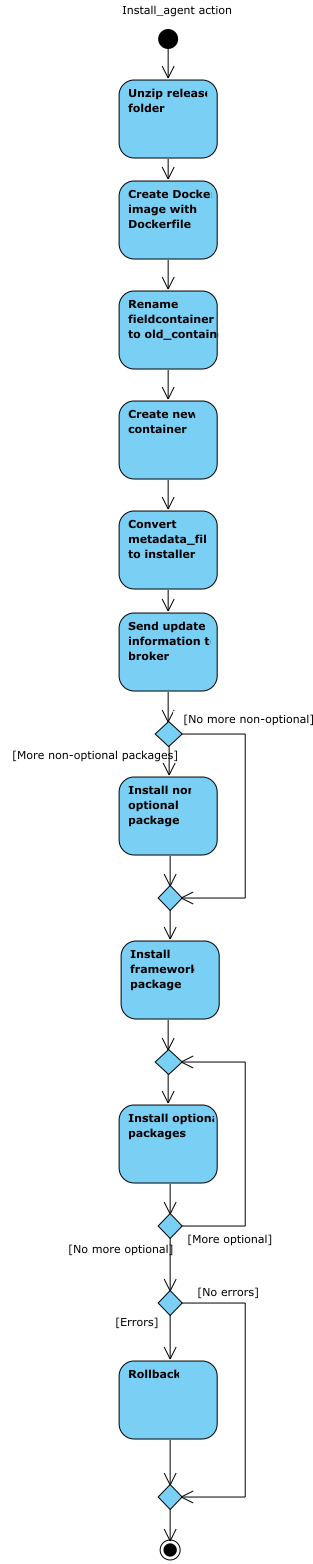
\includegraphics[scale=0.5]{afbeelding/flowcharts/installagent.png}
\caption{Acties van de installagent}
\label{fig:flow:install}
\end{figure}

\begin{figure}[!ht]
\centering
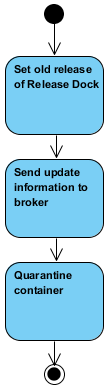
\includegraphics[scale=0.5]{afbeelding/flowcharts/rollback.png}
\caption{Rollback}
\label{fig:flow:rollback}
\end{figure}

\lstset{
    frame=single,
    breaklines=true,
    postbreak=\raisebox{0ex}[0ex][0ex]{\ensuremath{\color{red}\hookrightarrow\space}}
}

\chapter{Technologieën}
\lstinputlisting[caption={WiX Toolset installer}, label={list:wix}]{code/installer.wxs}

\lstinputlisting[caption={NSIS installer}, label={list:nsis}]{code/installer.nsi}
\chapter{Testscenario's}\label{sec:testen}
%\section{Cross-Platform container}\label{sec:crosscontainerscreen}
%\begin{sidewaysfigure}
%\includegraphics[width=\textwidth,height=\textheight,keepaspectratio]{afbeelding/architectuur.png}
%\centering
%\caption{Architectuur van het prototype}
%\label{fig:architectuur}
%\end{sidewaysfigure}

\section{Meerdere servers}
\begin{figure}[!ht]
\centering
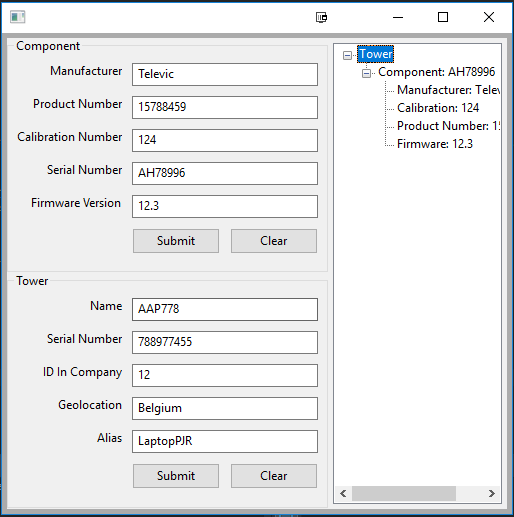
\includegraphics[scale=0.9]{afbeelding/testMultiServer/Setup.png}
\caption{Beschrijven van een client}
\label{fig:testServer:setup}
\end{figure}

\begin{sidewaysfigure}
\centering
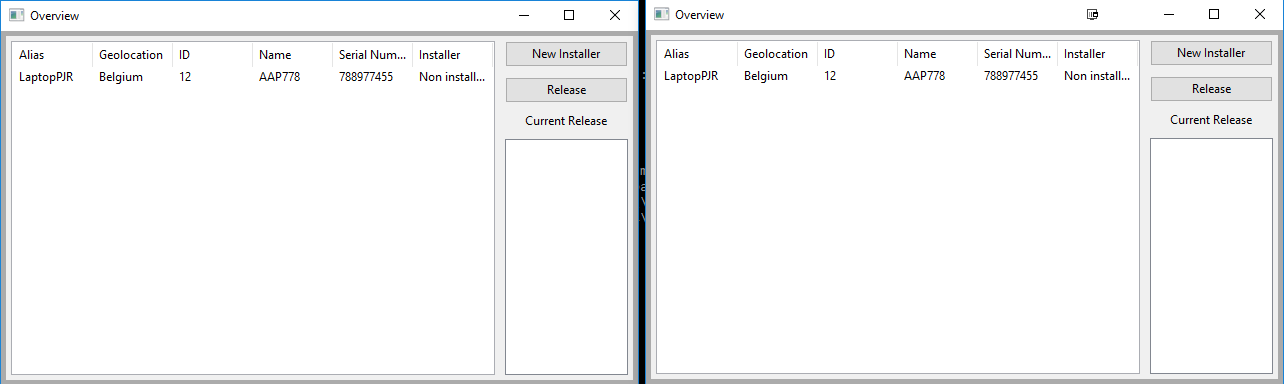
\includegraphics[width=\textwidth,height=\textheight,keepaspectratio]{afbeelding/testMultiServer/twoserverview.png}
\caption{Client overview van meerdere servers}
\label{fig:testServer:overview}
\end{sidewaysfigure}

\begin{sidewaysfigure}
\centering
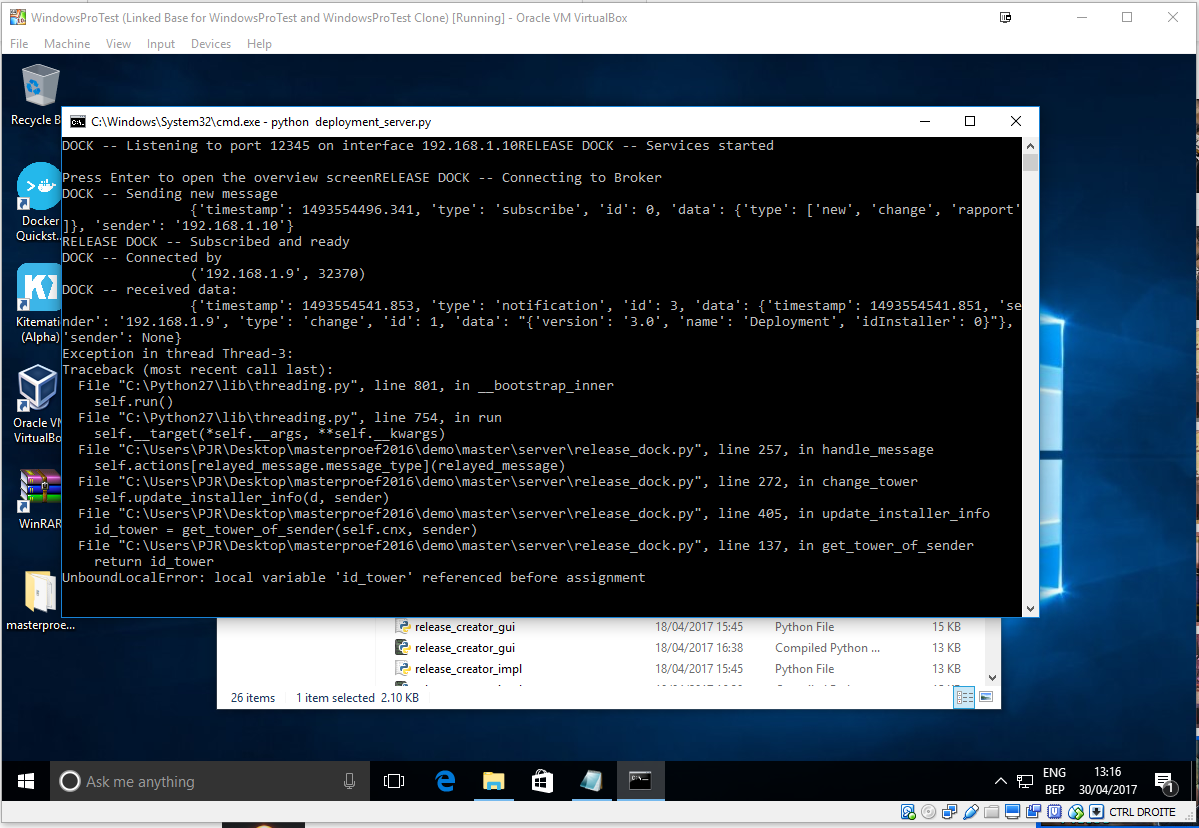
\includegraphics[width=\textwidth,height=\textheight,keepaspectratio]{afbeelding/testMultiServer/installatie.png}
\caption{Error tijdens het aanpassen van de field dock gegevens}
\label{fig:testServer:installation}
\end{sidewaysfigure}

\clearpage
\section{Meerdere clients}\label{sec:multiclientscreen}
\begin{sidewaysfigure}
\centering
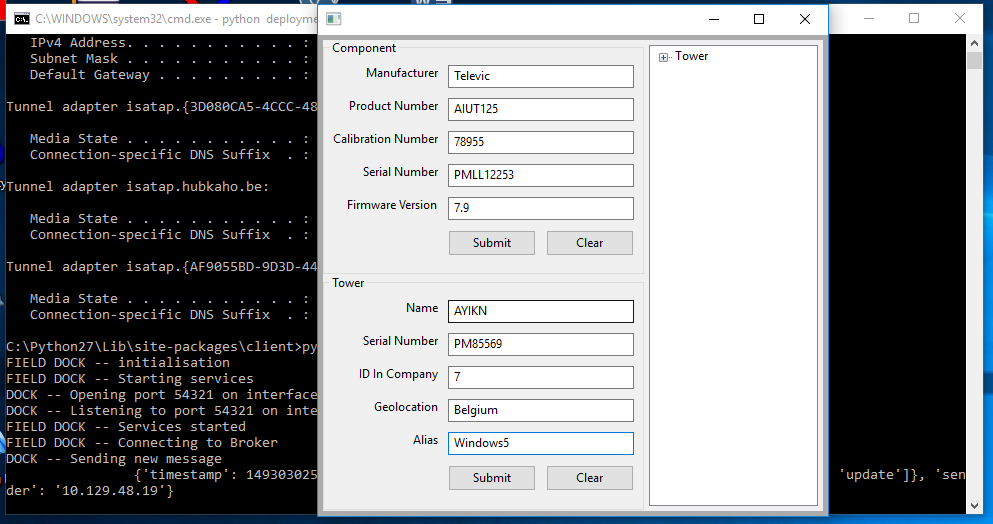
\includegraphics[width=\textwidth,height=\textheight,keepaspectratio]{afbeelding/testMultiClient/TorenBeschrijvenWindows.png}
\caption{Beschrijven van client in Windows}
\label{fig:testClient:windowsBeschrijving}
\end{sidewaysfigure}

\begin{sidewaysfigure}
\centering
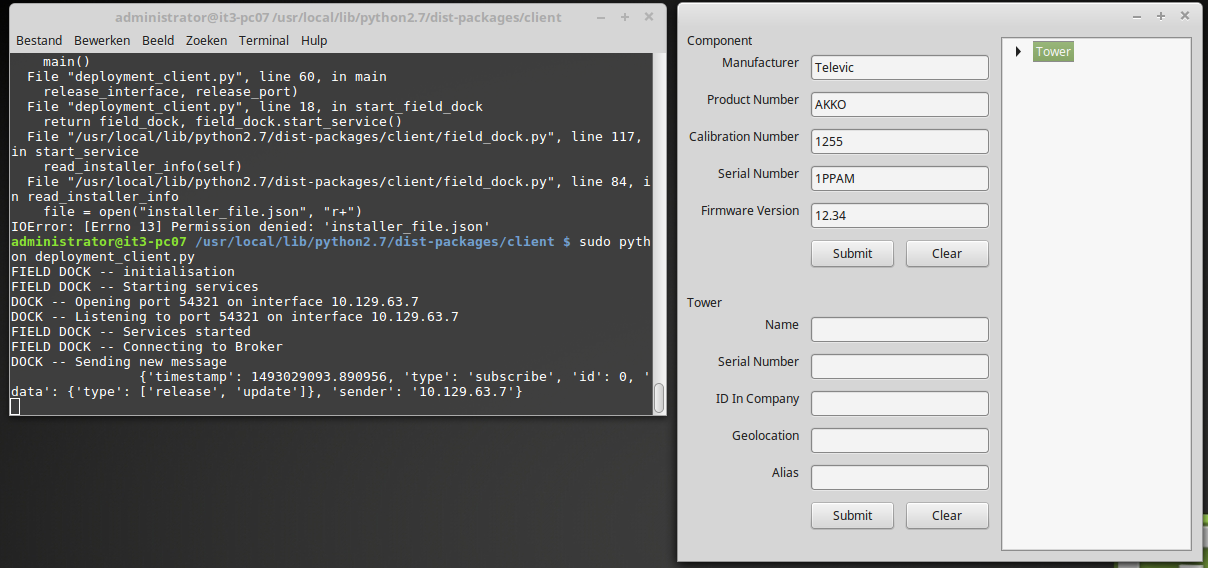
\includegraphics[width=\textwidth,height=\textheight,keepaspectratio]{afbeelding/testMultiClient/beschrijvenTorenLinux_cut.png}
\caption{Beschrijven van client in Linux}
\label{fig:testClient:linuxBeschrijving}
\end{sidewaysfigure}

\begin{figure}[!ht]
\centering
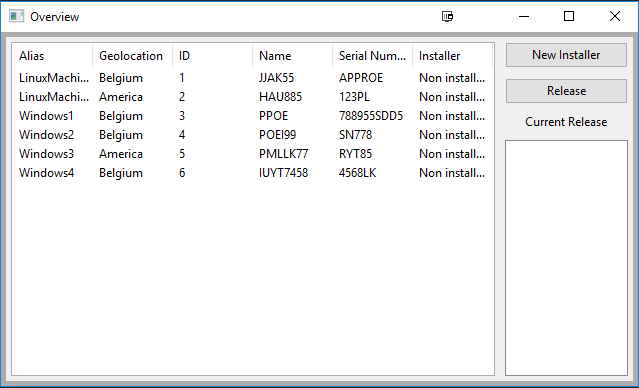
\includegraphics[scale=0.9]{afbeelding/testMultiClient/overview1.png}
\caption{Overview van de clients tijdens het toevoegen}
\label{fig:testClient:overviewTijdensToevoegen}
\end{figure}

\begin{figure}[!ht]
\centering
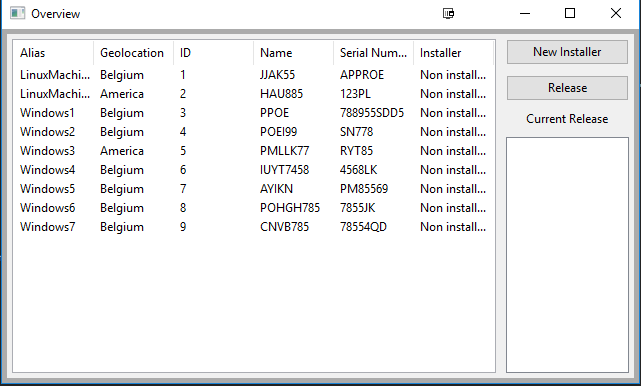
\includegraphics[scale=0.9]{afbeelding/testMultiClient/beforeRelease.png}
\caption{Overview van clients na toevoegen van de clients}
\label{fig:testClient:setup}
\end{figure}

\begin{figure}[!ht]
\centering
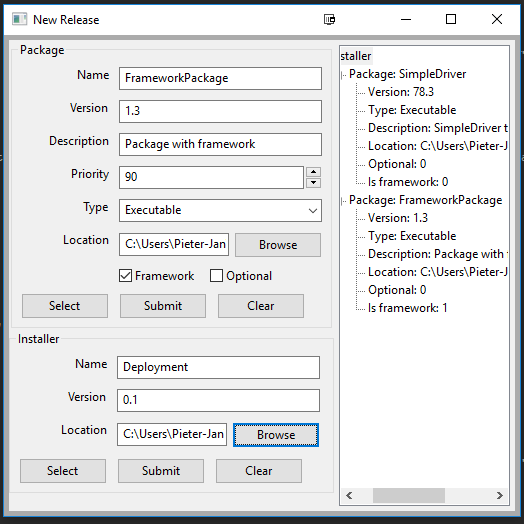
\includegraphics[scale=0.9]{afbeelding/testMultiClient/Release.png}
\caption{Creatie van een nieuwe installer}
\label{fig:testClient:newRelease}
\end{figure}

\begin{figure}[!ht]
\centering
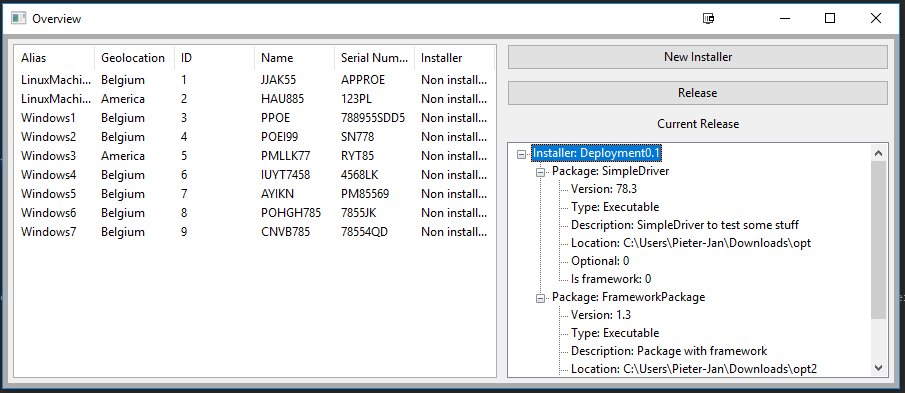
\includegraphics[width=\textwidth,keepaspectratio]{afbeelding/testMultiClient/JustBeforeRelease.png}
\caption{Overview van clients na creëren van een installer}
\label{fig:testClient:setupBeforeRelease}
\end{figure}

\begin{figure}[!ht]
\centering
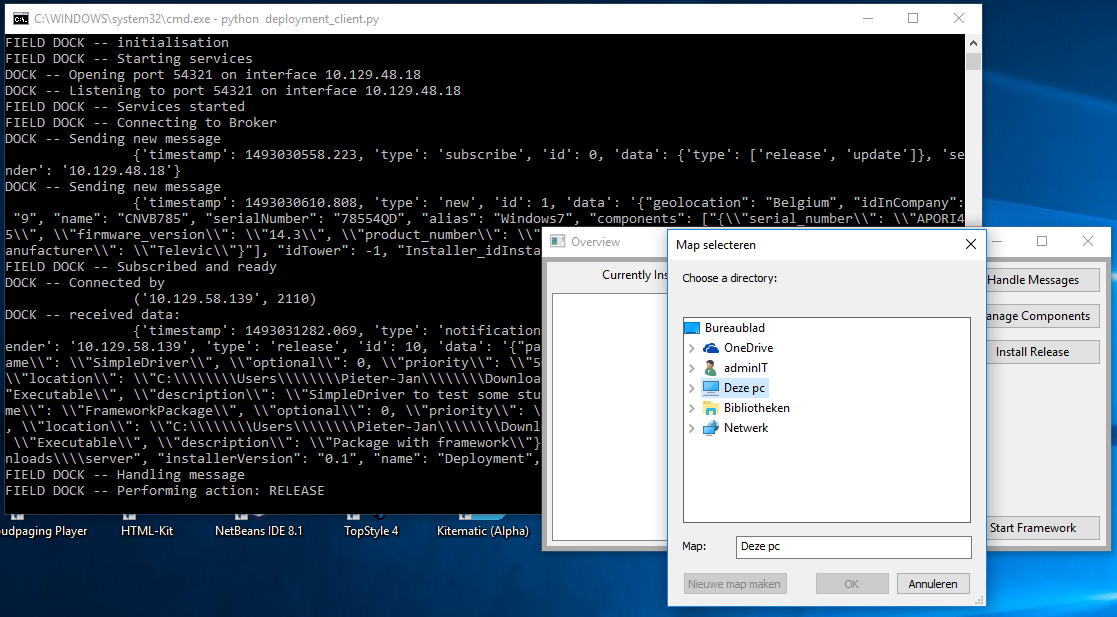
\includegraphics[width=\textwidth,keepaspectratio]{afbeelding/testMultiClient/MapSelection.png}
\caption{Selecteren van een folder voor de installer in te plaatsen}
\label{fig:testClient:mapSelection}
\end{figure}

\begin{sidewaysfigure}
\centering
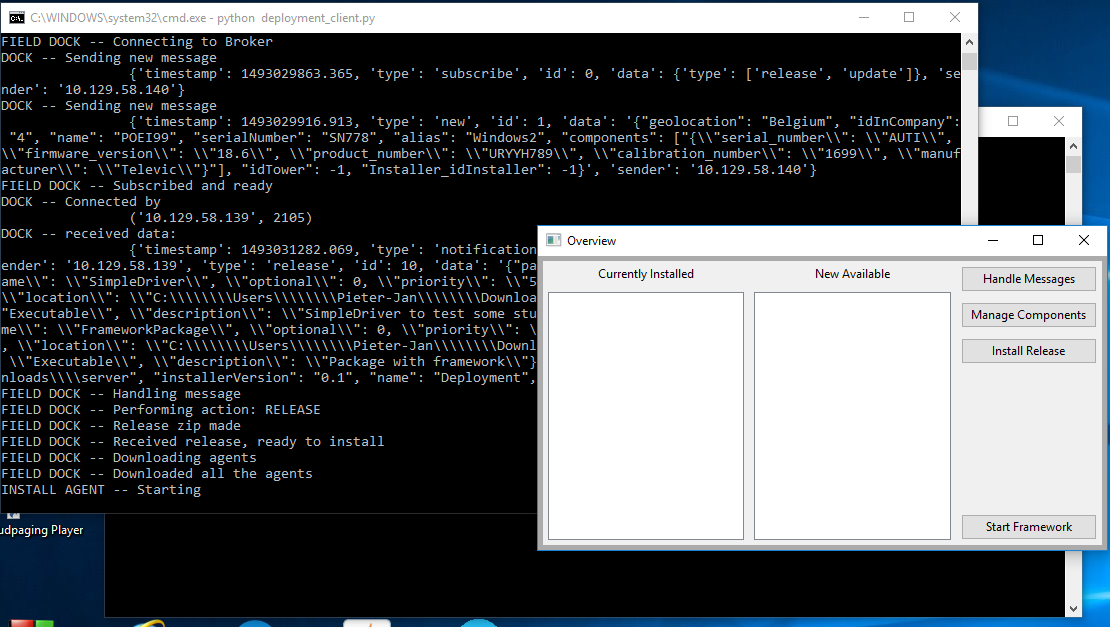
\includegraphics[width=\textwidth,height=\textheight,keepaspectratio]{afbeelding/testMultiClient/TijdensInstallatie_cut.png}
\caption{Output tijdens het installeren van de software}
\label{fig:testClient:tijdensInstallatie}
\end{sidewaysfigure}

\begin{figure}[!ht]
\centering
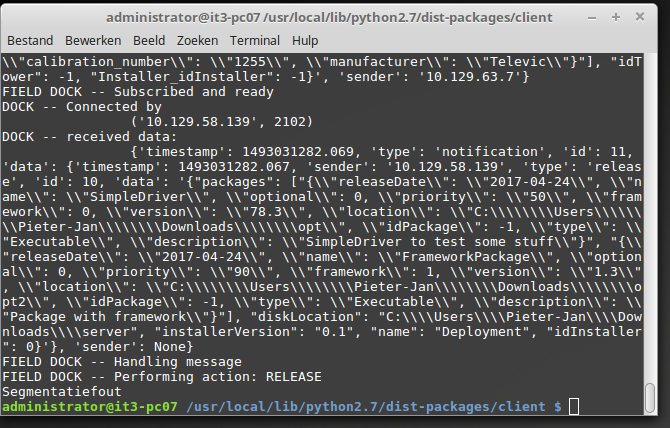
\includegraphics[width=\textwidth,keepaspectratio]{afbeelding/testMultiClient/LinuxInstallatieError.png}
\caption{Error tijdens het installeren van een installer in Linux}
\label{fig:testClient:linuxError}
\end{figure}

\begin{sidewaysfigure}
\centering
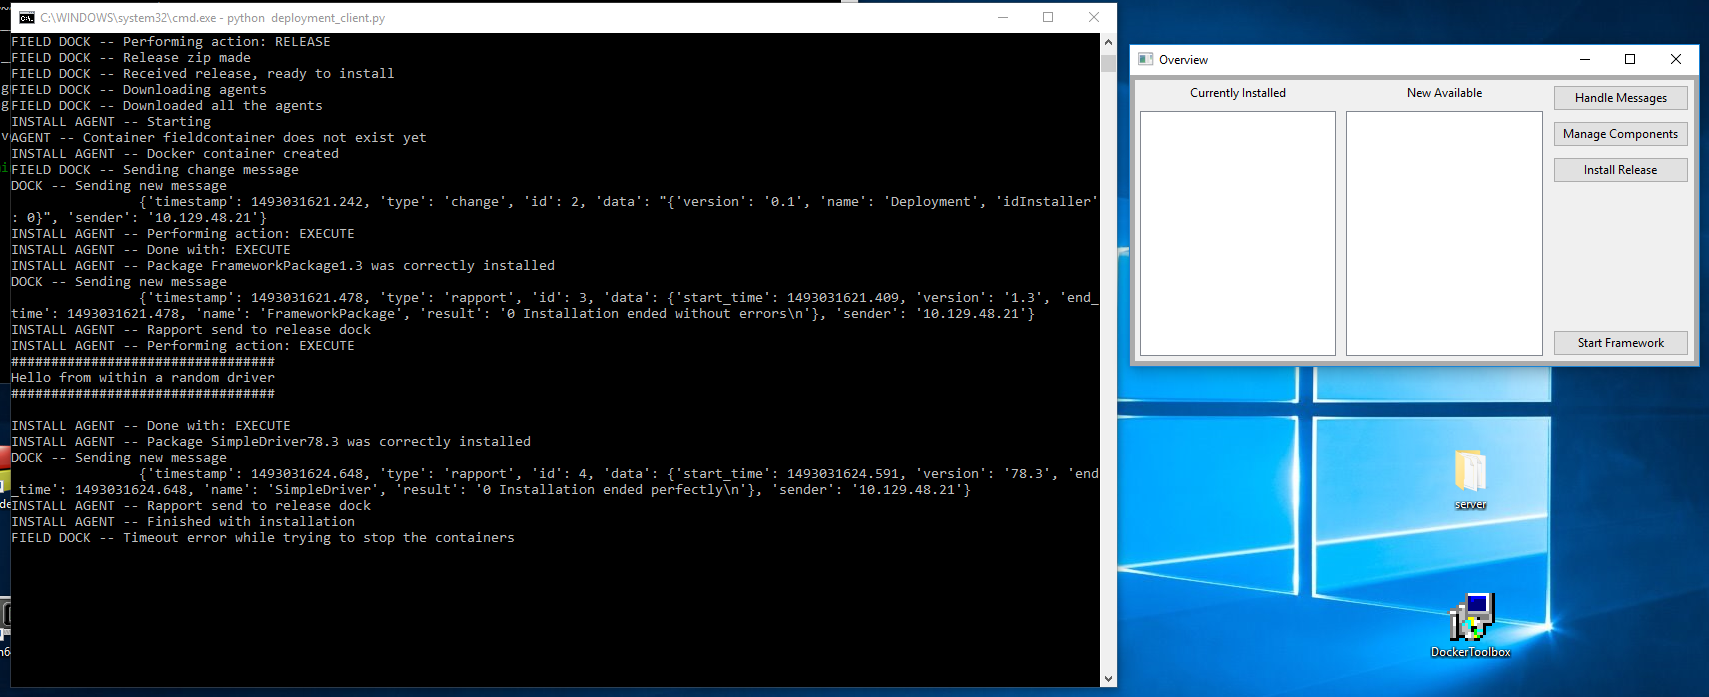
\includegraphics[width=\textwidth,height=\textheight,keepaspectratio]{afbeelding/testMultiClient/NaDeployment1_cut.png}
\caption{Installatie van een eerste installer}
\label{fig:testClient:installDeployment1}
\end{sidewaysfigure}

\begin{figure}[!ht]
\centering
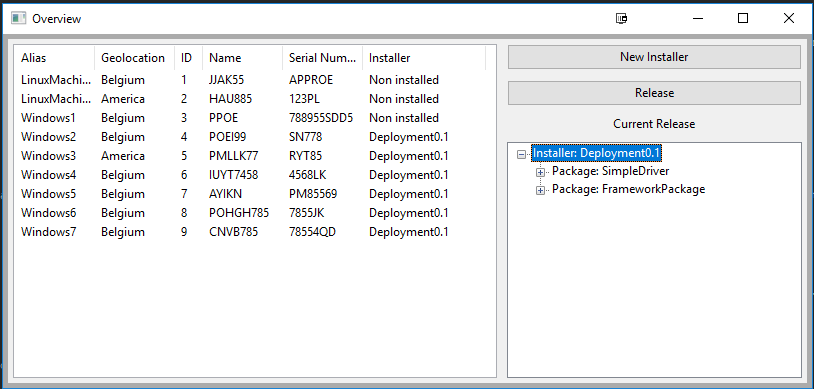
\includegraphics[width=\textwidth,keepaspectratio]{afbeelding/testMultiClient/OverviewNaRelease.png}
\caption{Overview van de clients na het verspreiden van de eerste installer}
\label{fig:testClient:overviewNaDeployment1}
\end{figure}

\begin{figure}[!ht]
\centering
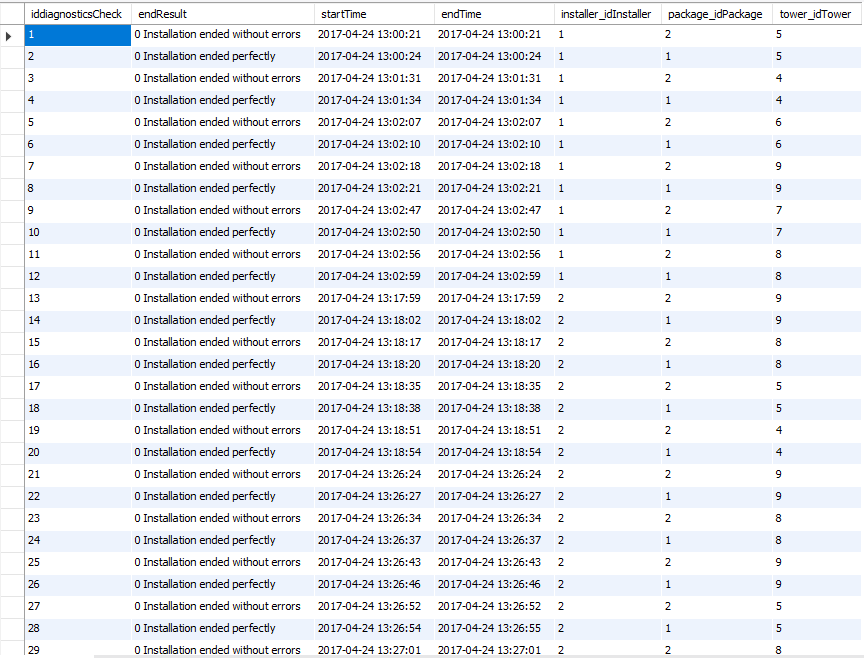
\includegraphics[width=\textwidth,keepaspectratio]{afbeelding/testMultiClient/RapportsDB.png}
\caption{Rapport tabel na uitvoeren van een installatie}
\label{fig:testClient:rapportDB}
\end{figure}

\begin{sidewaysfigure}
\centering
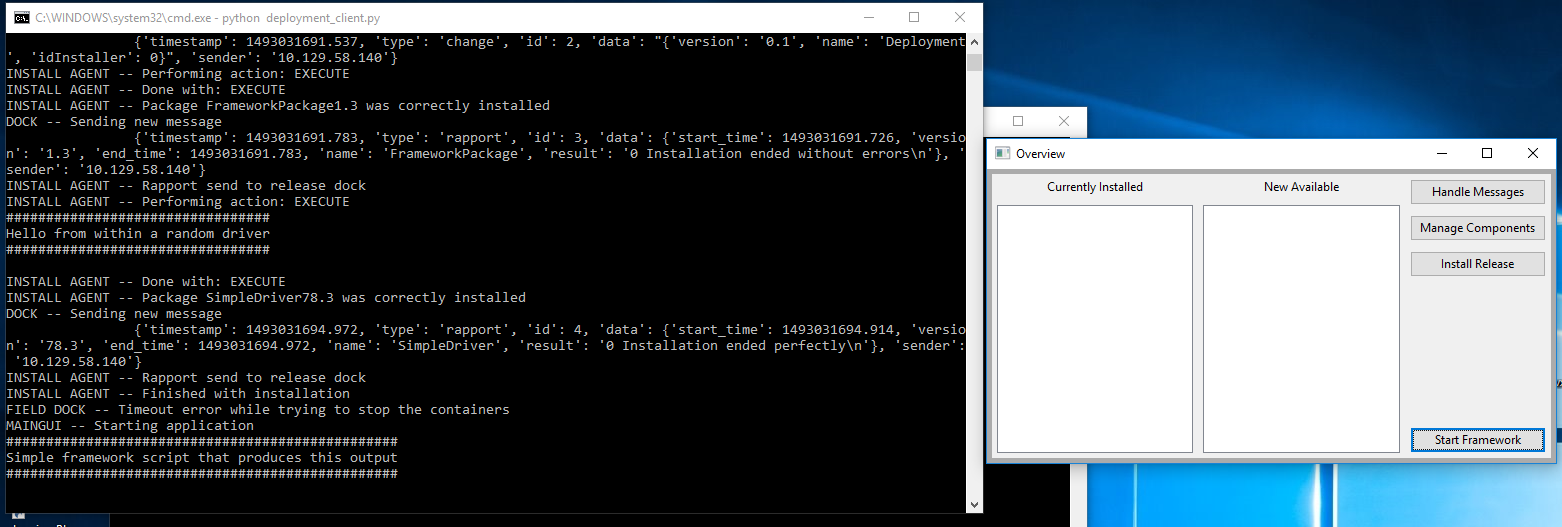
\includegraphics[width=\textwidth,height=\textheight,keepaspectratio]{afbeelding/testMultiClient/startFramework_cut.png}
\caption{Output na het opstarten van de geïnstalleerde software}
\label{fig:testClient:startFramework}
\end{sidewaysfigure}

\begin{sidewaysfigure}
\centering
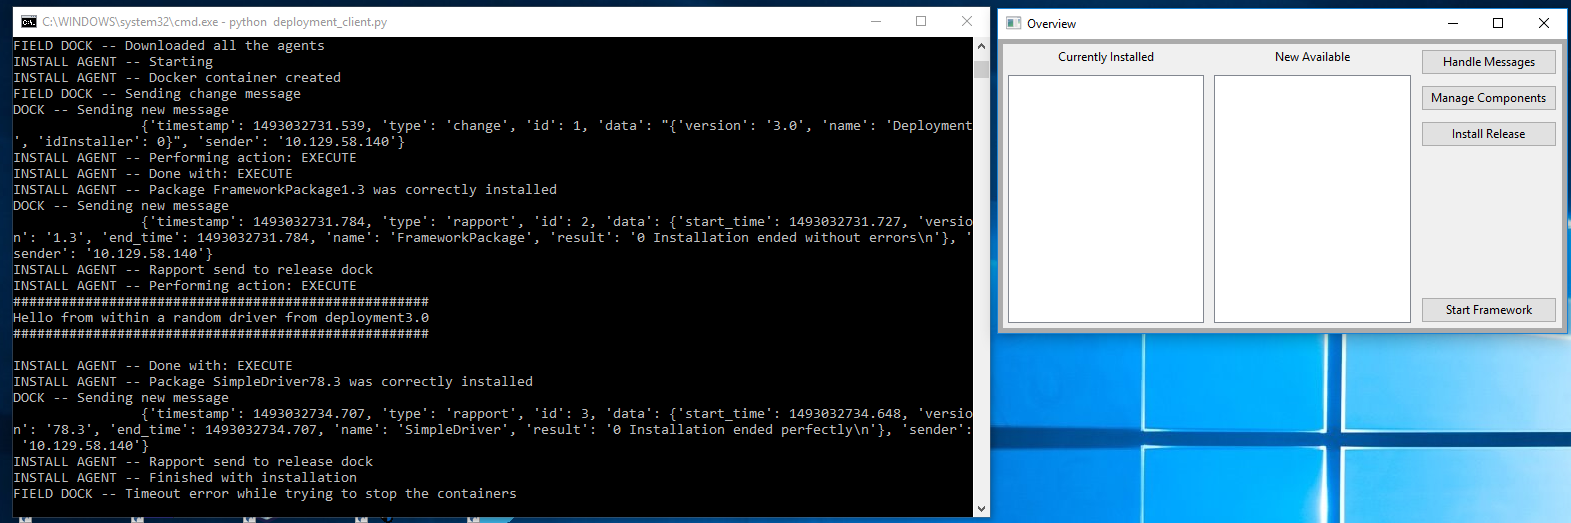
\includegraphics[width=\textwidth,height=\textheight,keepaspectratio]{afbeelding/testMultiClient/NaDeployment2_cut.png}
\caption{Installatie van een tweede installer}
\label{fig:testClient:installDeployment2}
\end{sidewaysfigure}

\begin{sidewaysfigure}
\centering
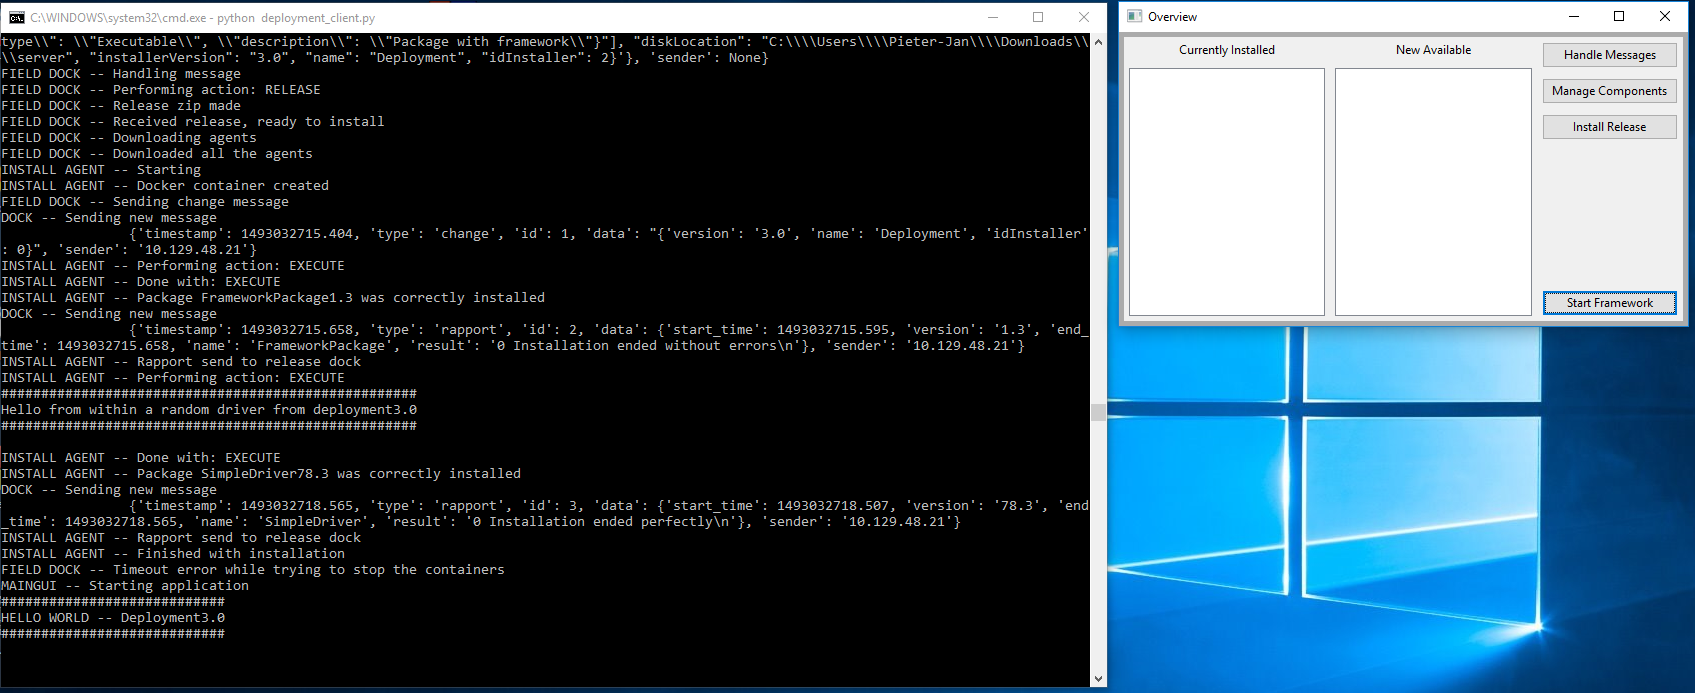
\includegraphics[width=\textwidth,height=\textheight,keepaspectratio]{afbeelding/testMultiClient/StartNaDeployment2_cut.png}
\caption{Output na het opstarten van de geïnstalleerde software}
\label{fig:testClient:startFramework2}
\end{sidewaysfigure}

\begin{figure}[!ht]
\centering
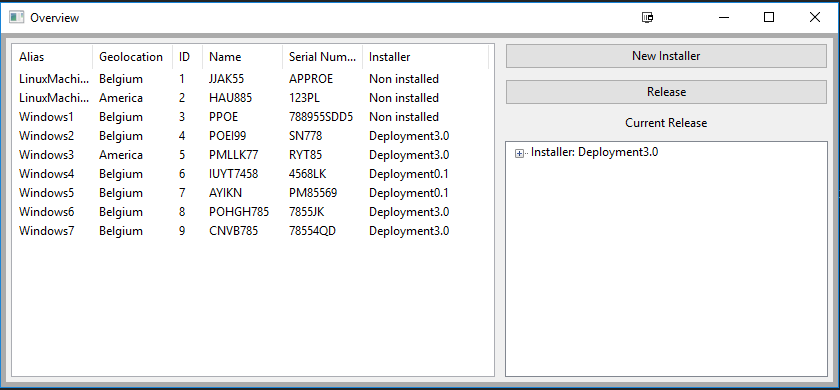
\includegraphics[width=\textwidth,keepaspectratio]{afbeelding/testMultiClient/OverviewNaDeployment2.png}
\caption{Overview van de clients na het verspreiden van een tweede installer}
\label{fig:testClient:overviewNaDeployment2}
\end{figure}

\clearpage
\section{Slecht werkend pakket}\label{sec:badPackage}
\begin{figure}[!ht]
\centering
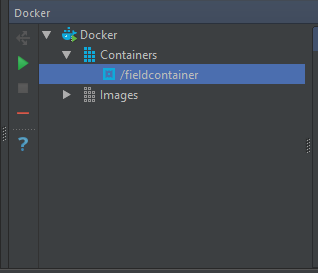
\includegraphics[scale=1]{afbeelding/badPackage/begin.png}
\caption{Opsomming van aanwezige containers voor het installatieproces}
\label{fig:badPackage:begin}
\end{figure}

\begin{figure}[!ht]
\centering
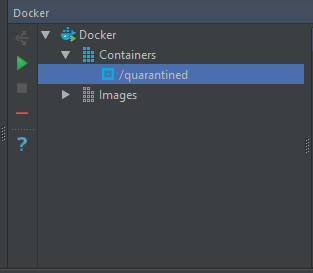
\includegraphics[scale=1]{afbeelding/badPackage/einde.png}
\caption{Opsomming van aanwezige containers na het installatieproces}
\label{fig:badPackage:einde}
\end{figure}

\begin{sidewaysfigure}
\centering
\includegraphics[scale=0.9]{afbeelding/badPackage/installatieProces.png}
\caption{Output tijdens het installatieproces}
\label{fig:badPackage:tijdens}
\end{sidewaysfigure}

\clearpage
\section{Netwerk monitoring}\label{sec:network}
\begin{sidewaysfigure}
\centering
\includegraphics[scale=0.9]{afbeelding/network/broker_notification.png}
\caption{Doorsturen van een notificatie}
\label{fig:network:notification}
\end{sidewaysfigure}

\begin{sidewaysfigure}
\centering
\includegraphics[scale=0.9]{afbeelding/network/installatieDoorsturen.png}
\caption{Doorsturen van een installer en agenten naar een field dock}
\label{fig:network:installatie}
\end{sidewaysfigure}

\begin{sidewaysfigure}[!ht]
\centering
\includegraphics[scale=0.9]{afbeelding/network/rapport.png}
\caption{Doorsturen van een rapport naar de broker}
\label{fig:network:rapport}
\end{sidewaysfigure}

\begin{figure}[!ht]
\centering
\includegraphics[scale=1]{afbeelding/network/statistics.png}
\caption{Algemene statistieken bij het verzenden van een installer}
\label{fig:network:stats}
\end{figure}

% Bijlage met daarin het wetenschappelijk artikel
%%%%%%%%%%%%%%%%%%%%%%%%%%%%%%%%%%%%%%%%%%%%%%%%%%
\chapter{Beschrijving van deze masterproef in de vorm van een wetenschappelijk artikel}
%\includepdf{artikel.pdf}

% Bijlage met daarin de poster
%%%%%%%%%%%%%%%%%%%%%%%%%%%%%%%
\chapter{Poster}
\includepdf{poster.pdf}

\includepdf{back_fiiw_gent.pdf}
% \includepdf{back_fiiw_ghent_eng.pdf} % For the english version

\end{document}
